\documentclass[12pt]{article}

\usepackage{upgreek}

\usepackage{amsmath}

\usepackage{graphicx}
\graphicspath{ {imgs/} }

\usepackage{dsfont}

\usepackage{mathtools}

\usepackage{hyperref}

\usepackage[utf8]{inputenc}

\usepackage{mathtools}

\usepackage{textcomp}

\usepackage[english]{babel}

\usepackage{tikz}

\usepackage{tcolorbox}

\usepackage{amsthm,amssymb}

\setlength{\parindent}{0cm}

\renewcommand\qedsymbol{$\blacksquare$}

\usepackage{fancyhdr}
 
\pagestyle{fancy}
\fancyhf{}
\fancyhead[LE,RO]{Graph Theory -- Fall 2017}
\fancyhead[RE,LO]{Joshua Concon}
\fancyfoot[CE,CO]{\leftmark}
\fancyfoot[LE,RO]{\thepage}


\begin{document}

\title{MATC32: Graph Theory\\ Lecture Notes}
\date{University of Toronto Scarborough -- Fall 2017}
\author{Joshua Concon}
\maketitle
Pre-reqs are MATB24, which is the second course on linear algebra at UTSC.
Instructor is Dr. Louis de Thanhoffer de Volcsey. I highly recommend sitting at the front since he likes to teach with the board. If you find any problems in these notes, feel free to contact me at conconjoshua@gmail.com.

\tableofcontents

\pagebreak

\section{Tuesday, September 5, 2017}

\subsection{The Seven Bridges of Konigsberg}

So basically there's this city called Konigsberg where a river flows through, and because of that, there are 7 bridges in the city. The bridges look like this:\\
\\
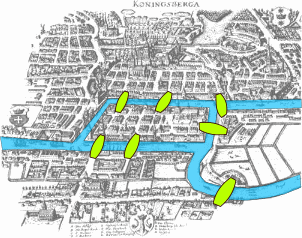
\includegraphics{Konigsberg_bridges}\\
\\

There problem that came up is whether or not it was possible to walk through every bridge in the city once in the same walk. This problem was eventually solved by Euler.\\
\\
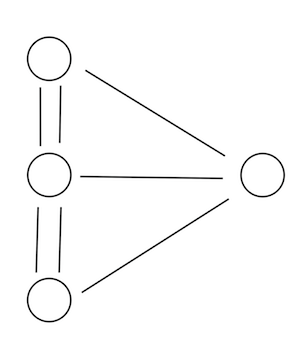
\includegraphics{Konigsberg_bridges_graph}\\
\\
It can be simplified to this. This is called a 'Graph', the circles are called 'nodes' or 'vertices' and the lines are called 'edges'. The different parts of the city are represented by the nodes and the bridges are represented by the edges.\\
\\
\begin{tcolorbox}[title=Definition: Graph ($G$)]
	\begin{enumerate}
		\item{Contains a set $V(G) =$ the set of nodes}
		\item{Contains a set $E(G) =$ the set of edges}
	\end{enumerate}
	A graph is called \textbf{Simple} if the graph has no loops and does not have multiple edges (i.e. Each edge is an unordered pair of distinct vertices).\\
	A graph is called a \textbf{Loop} if there is an edge that connects a vertex to itself.
\end{tcolorbox}

\begin{tcolorbox}[title=Definition: Path]
	A set of edges denoted by vertices $v_1, v_2, ..., v_n$ where there is a node between every edge between $v_i$ and $v_{i+1}$ $\forall i, 1 \leq i \leq n-1$
\end{tcolorbox}

\subsection{(Outline) Solution to Konigsberg}

Assume the graph has a path containing all edges $u_1,...,u_n$.\\
\\
Consider a vertex that isn't the first or last vertex travelled in the path (i.e. any vertex excluding $u_1$ and $u_n$).\\
\\
There must be an even number of edges for each of the nodes in between the edges in the path (excluding the first and the last node visited, unless the first and the last node visited are the same node).\\
\\
Since there are an odd number of adjacent nodes for all 4 nodes, this path does not exist. Therefore, there is no solution to Konigsberg.

\newpage

\section{Friday, September 8, 2017}

\subsection{Graphs}

\begin{tcolorbox}[title=Definition: Graphs]
	A graph $G$ consists of 2 (finite) sets:
	\begin{itemize}
		\item{$V(G)$ : vertex set}
		\item{$E(G)$ : edge set}
	\end{itemize}

	Together with an assignment from $E(G)$ to the set of subsets $V(G)$, where the subset is of size 1 or 2, containing the node(s) at the ends of the endpoints of each edge.
\end{tcolorbox}

If an edge has the same node at both of it's endpoints, it is called a \textbf{loop}.\\
\\
If 2 vertices are endpoints of more than one edge, we say that they are \textbf{multiply-edged}.\\
\\
A graph without multiply-edged vertices is called \textbf{simple}.\\
\\
\underline{Example:}


\includegraphics[scale=0.125]{lec2-1}

$$E(G) = \{ e_1, ... , e_7 \}$$
$$V(G) = \{ N_1, ... , N_4 \}$$

some of the assignments of $E(G) \mapsto V(G)$ include:
$$e_5 \mapsto \{ N_1, N_4 \}$$

\textbf{Adjacent edges} are edges with a vertex that is a common endpoint.

\subsection{Graph Theory Applications}

\subsubsection{Uber}

$$V = \text{People Using Uber (both drivers and passengers)}$$
$$E = \text{If it is realistic for a driver to pick up a person}$$

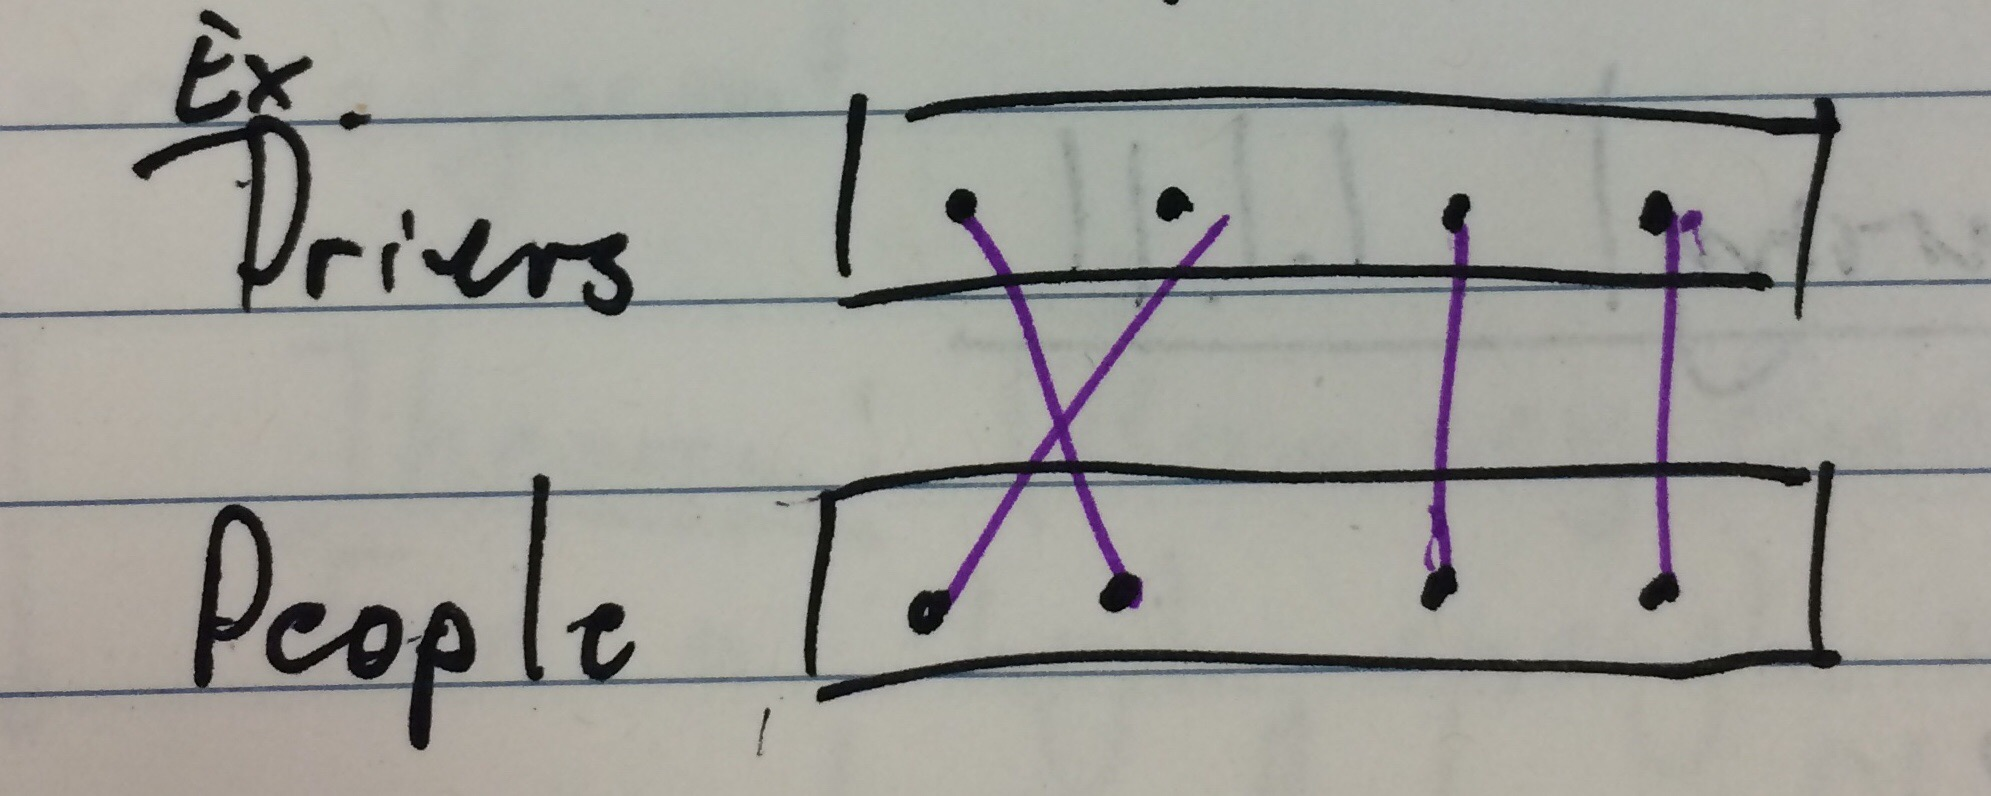
\includegraphics[scale=0.125]{lec2-2}

\begin{tcolorbox}[title=Definition: Matching]
	A \textbf{matching} in a group is a set of edges, none of which are adjacent
\end{tcolorbox}

\underline{Note:} $V(G) = S_1 \sqcup S_2$ and there are no edges between of $S_1$ with respect to $S_2$ ($\sqcup$ : refers to a union between two disjoint sets).\\
\\
These two sets $S_1, S_2$ are independent sets\\
\\
A \textbf{bipartite} graph has $V(G) = S_1 \sqcup S_2$ where both $S_1, S_2$ are independent.

\subsubsection{Monge's Theorem (on matching)}

Split a deck of 52 cards into 13 piles of 4, is it always possible to count an ace,2,3,...., Jack, Queen, King using 1 card drawn from each pile?

\subsubsection{Marriage (Stable) Problem}

Matching $n$ men with $n$ women

\subsubsection{Scheduling (Graph Colouring)}

Let $V$ represent different courses, and edges between courses mean that a student can take both courses at the same time. The problem is to reduce the edges between vertices with the same label or colour.\\
\\
$X(G)$ is the chromatic number of a graph $G$ and is the minimum number of colours needed to colour a graph without the edges having endpoints with two vertices of the same colour. To distribute these colours, there is a mapping from $V(G) \mapsto C$ where $C$ is a set of colours.\\
\\
\underline{Statement:} In a room of people, we can always be certain that 3 people either know each other or are all strangers for a room of 6+ people. So if we represent the people in the room as vertices in a non simple graph, and edge connections between people as the two unique people at the endpoints refer to familiarity or unfamiliarity, then you can always form a triangle with the edges.\\
\\
This is the proof of $R(3,3)=6$ for Ramsey's Theorem.\\
\\
\begin{tcolorbox}[title=Definition: Complete Graph]
	A Complete Graph is a simple graph where any 2 vertices are adjacent.
\end{tcolorbox}

A \textbf{clique} is a subset of vertices $C$ such that all vertices are adjacent.

\begin{tcolorbox}[title=Theorem: Ramsey's theorem]
	For a high enough number $R(n,m)$, we can guarantee that after colouring a complete graph of $m$ vertices with $2$ colours (in any way), there will be a clique of $n$ vertices of the same colour.
\end{tcolorbox}

\subsubsection{Network Problems}

A path is a series of vertices $v_1, .., v_n$ where $v_i$ and $v_{i+1}$ are adjacent for all $i, 1 \leq i \leq n-1$.\\
\\
Say 2 vertices are \textbf{connected} if there exists a path between them.\\
\\
Cutting number of 2 vertices $m,n$ are the amount of vertices that need to be removed such that vertices $m,n$ are not connected.
\\
\\
\underline{Example:}\\
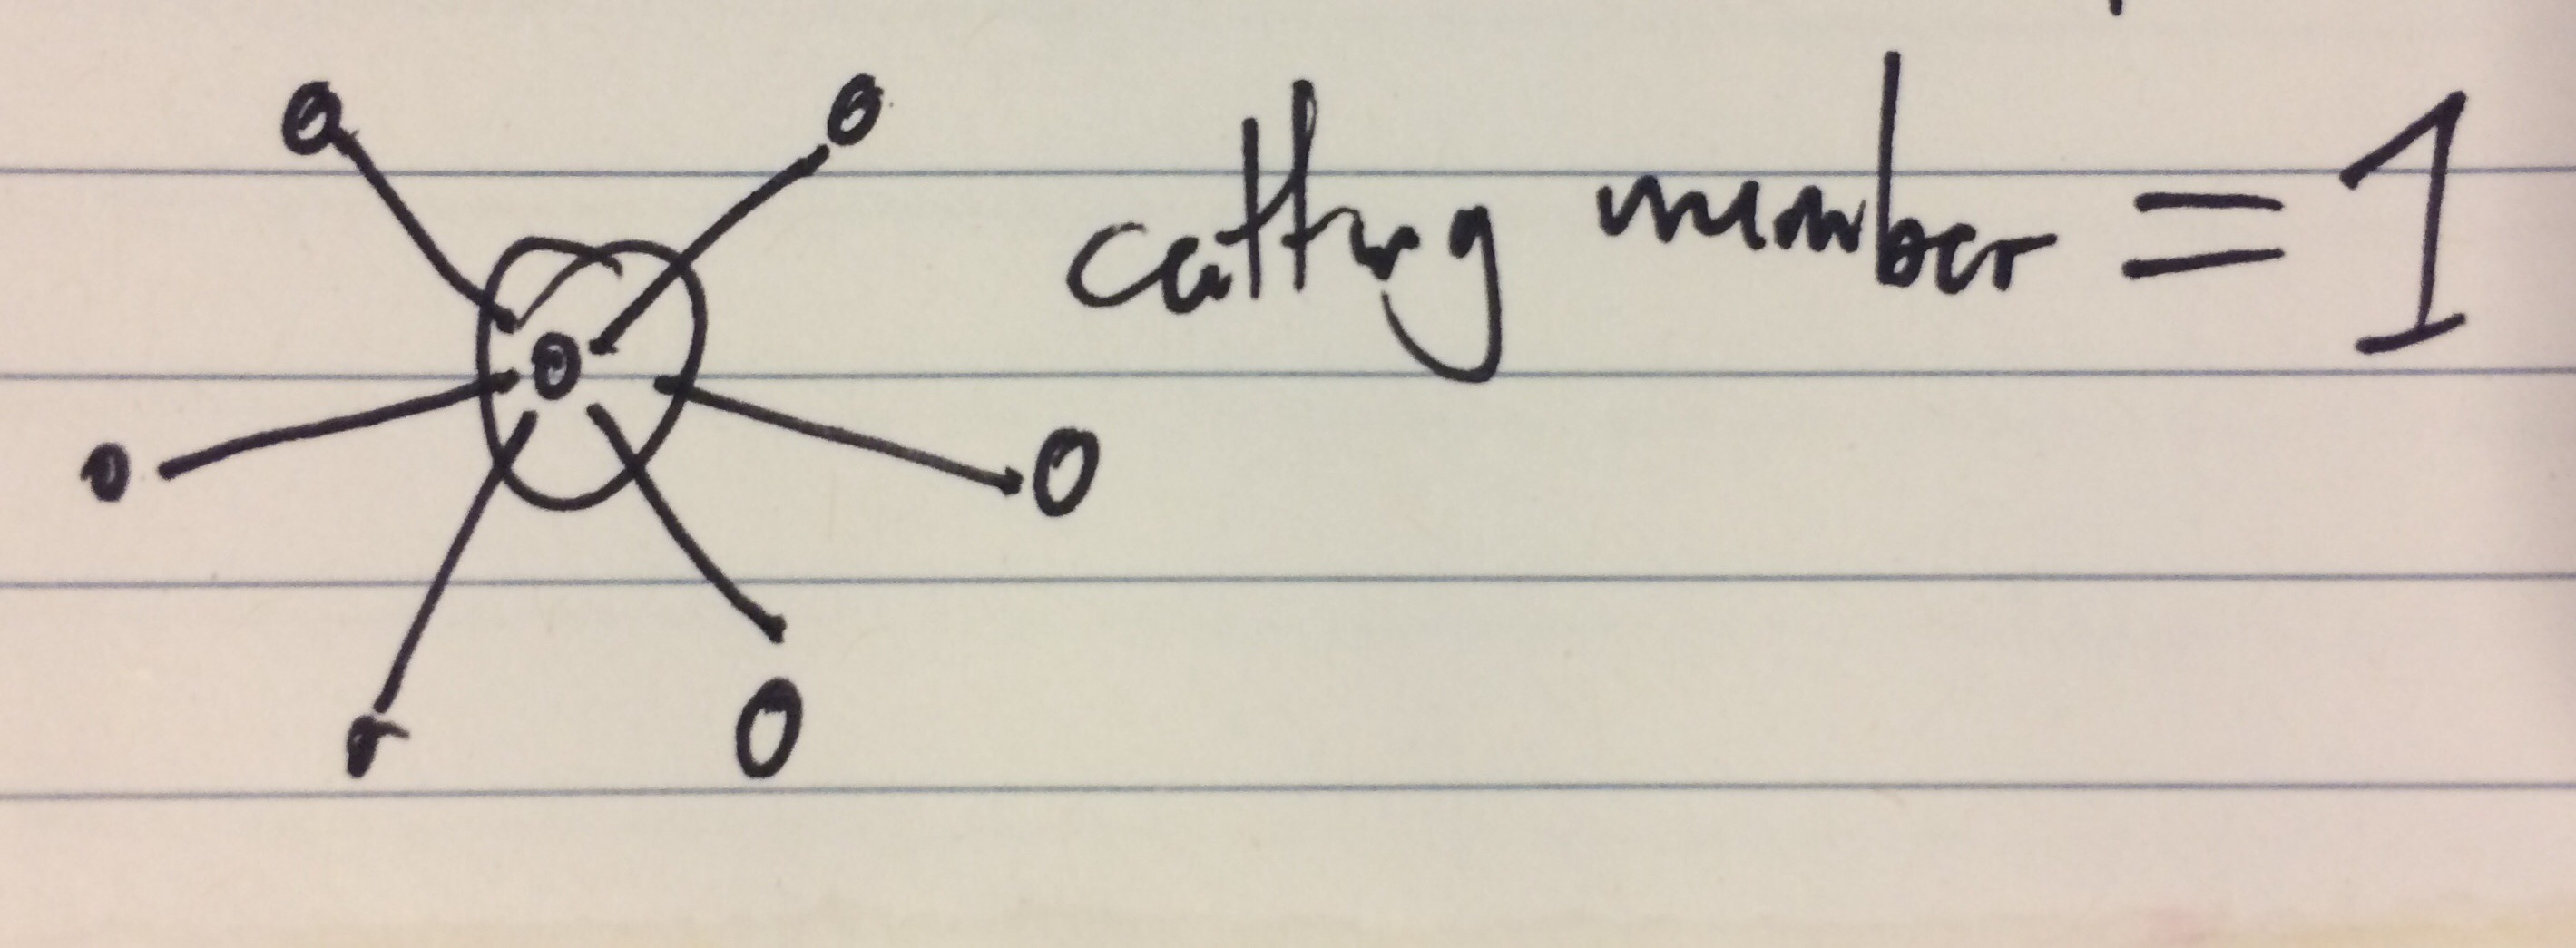
\includegraphics[scale=0.125]{lec2-3}

\subsubsection{Uber (Pathfinding)}

Pathfinding is a graph problem where $V$ represents all the intersections of a map and $E$ is all the roads. For a path $v_1, ... ,v_n$, the length is the number $m$, which is the sum of all the edge weights $\geq 0$, and for 2 connected vertices, we are trying to find the path of the least length. Dijsktra's Algorithm solves this problem.

\subsection{Morphism}

A morphism of graphs $G \mapsto G'$ consists of 2 functions:
\begin{itemize}
	\item{$\gamma_1 : V(G) \mapsto V(G')$}
	\item{$\gamma_2 : E(G) \mapsto E(G')$}
\end{itemize}

$\forall e$, if $e \in E(G)$ has endpoints $v_1, v_2$, this implies that $\gamma_2 (e)$ has endpoints $\gamma_1 (v_1), \gamma_1 (v_2)$.\\
\\
\begin{tcolorbox}
	Note: This definition is more general than the book.
\end{tcolorbox}

An isomorphism is a morphism such that $\gamma_1, \gamma_2$ are both bijective.
\\
\\
\underline{Example of a morphism:} (Note that $\simeq$ denotes a morphism)\\
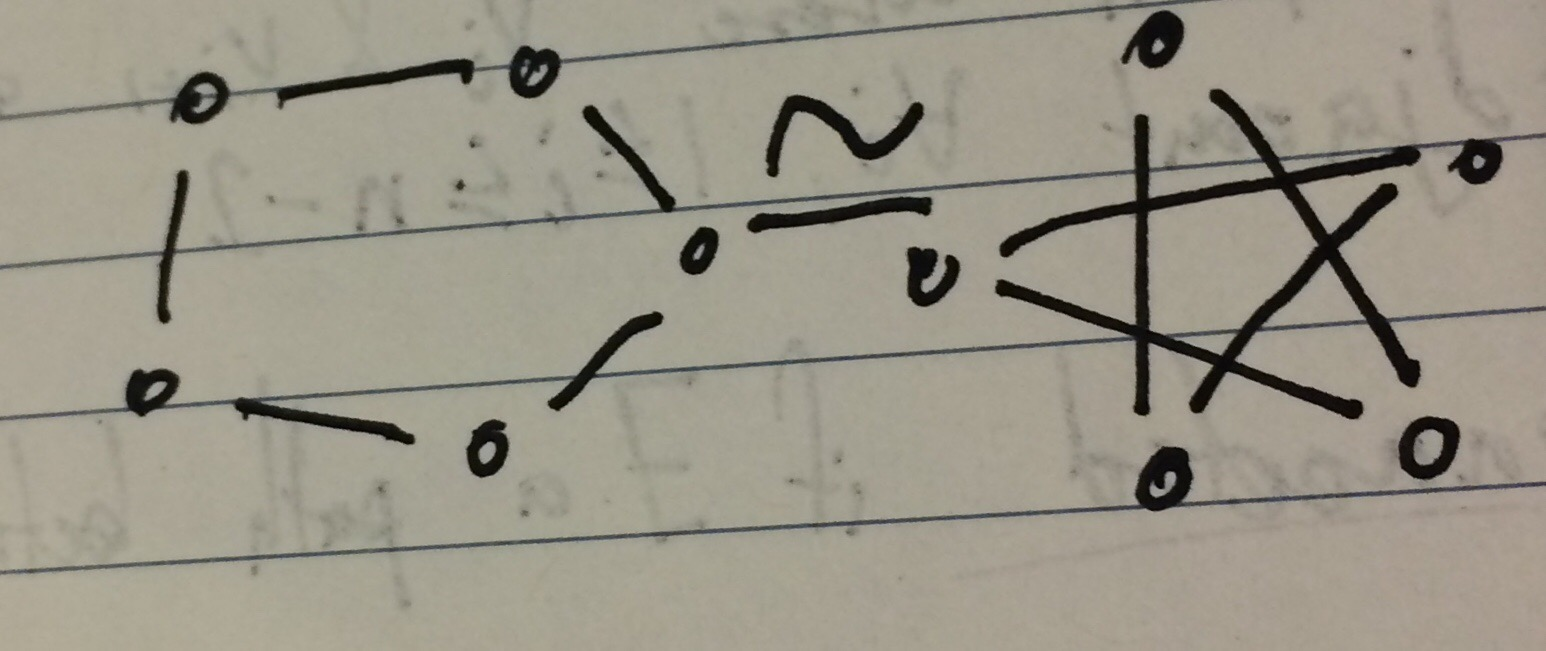
\includegraphics[scale=0.125]{lec2-4}

\newpage

\section{Tuesday, September 12, 2017}

\subsection{More Morphism}

\begin{tcolorbox}[title=Observation 1]
	if $G'$ is simple, there exists a morphism $G \mapsto G'$ and so $\gamma_1 : V(G) \mapsto V(G')$ such that if $e\in E(G)$ has endpoints $v_1, v_2$, then $\gamma_1 (v_1), \gamma_1 (v_2)$ are adjacent.
\end{tcolorbox}

A \textbf{subgraph} of $G$ is a subset $V' \subset V$, $E' \subset E$ such that $Id: (V', E') \mapsto G$ is a morphism.\\
\\
An \textbf{isomorphism} is when a morphism $G \mapsto G'$ is bijective (That there is a one to one relationship between $E \mapsto E'$ and $V \mapsto V'$)\\
\\
\underline{Exercise:} if $(\gamma_1, \gamma_2) : G \mapsto G'$ is an isomorphism, then $(\gamma_1^{-1}, \gamma_2^{-1}) : G' \mapsto G$\\
\\
\underline{Recall:} Bijective implies injective and surjective.

\begin{tcolorbox}[title=Definition: Complement of Simple Graphs]
	The complement of a simple graph $G$ is $\overset{\_\_\_}{G} = (\overset{\_\_\_}{V},\overset{\_\_\_}{E})$ where $V(\overset{\_\_\_}{G}) = V(G)$ and $\overset{\_\_\_}{E}$ does not have any edge in $E$, but if $v_1,v_2 \in V$ are not adjacent, then $v_1,v_2$ are adjacent in $\overset{\_\_\_}{G}$ for all $v_1,v_1 \in V$
\end{tcolorbox}

\underline{Example:}\\
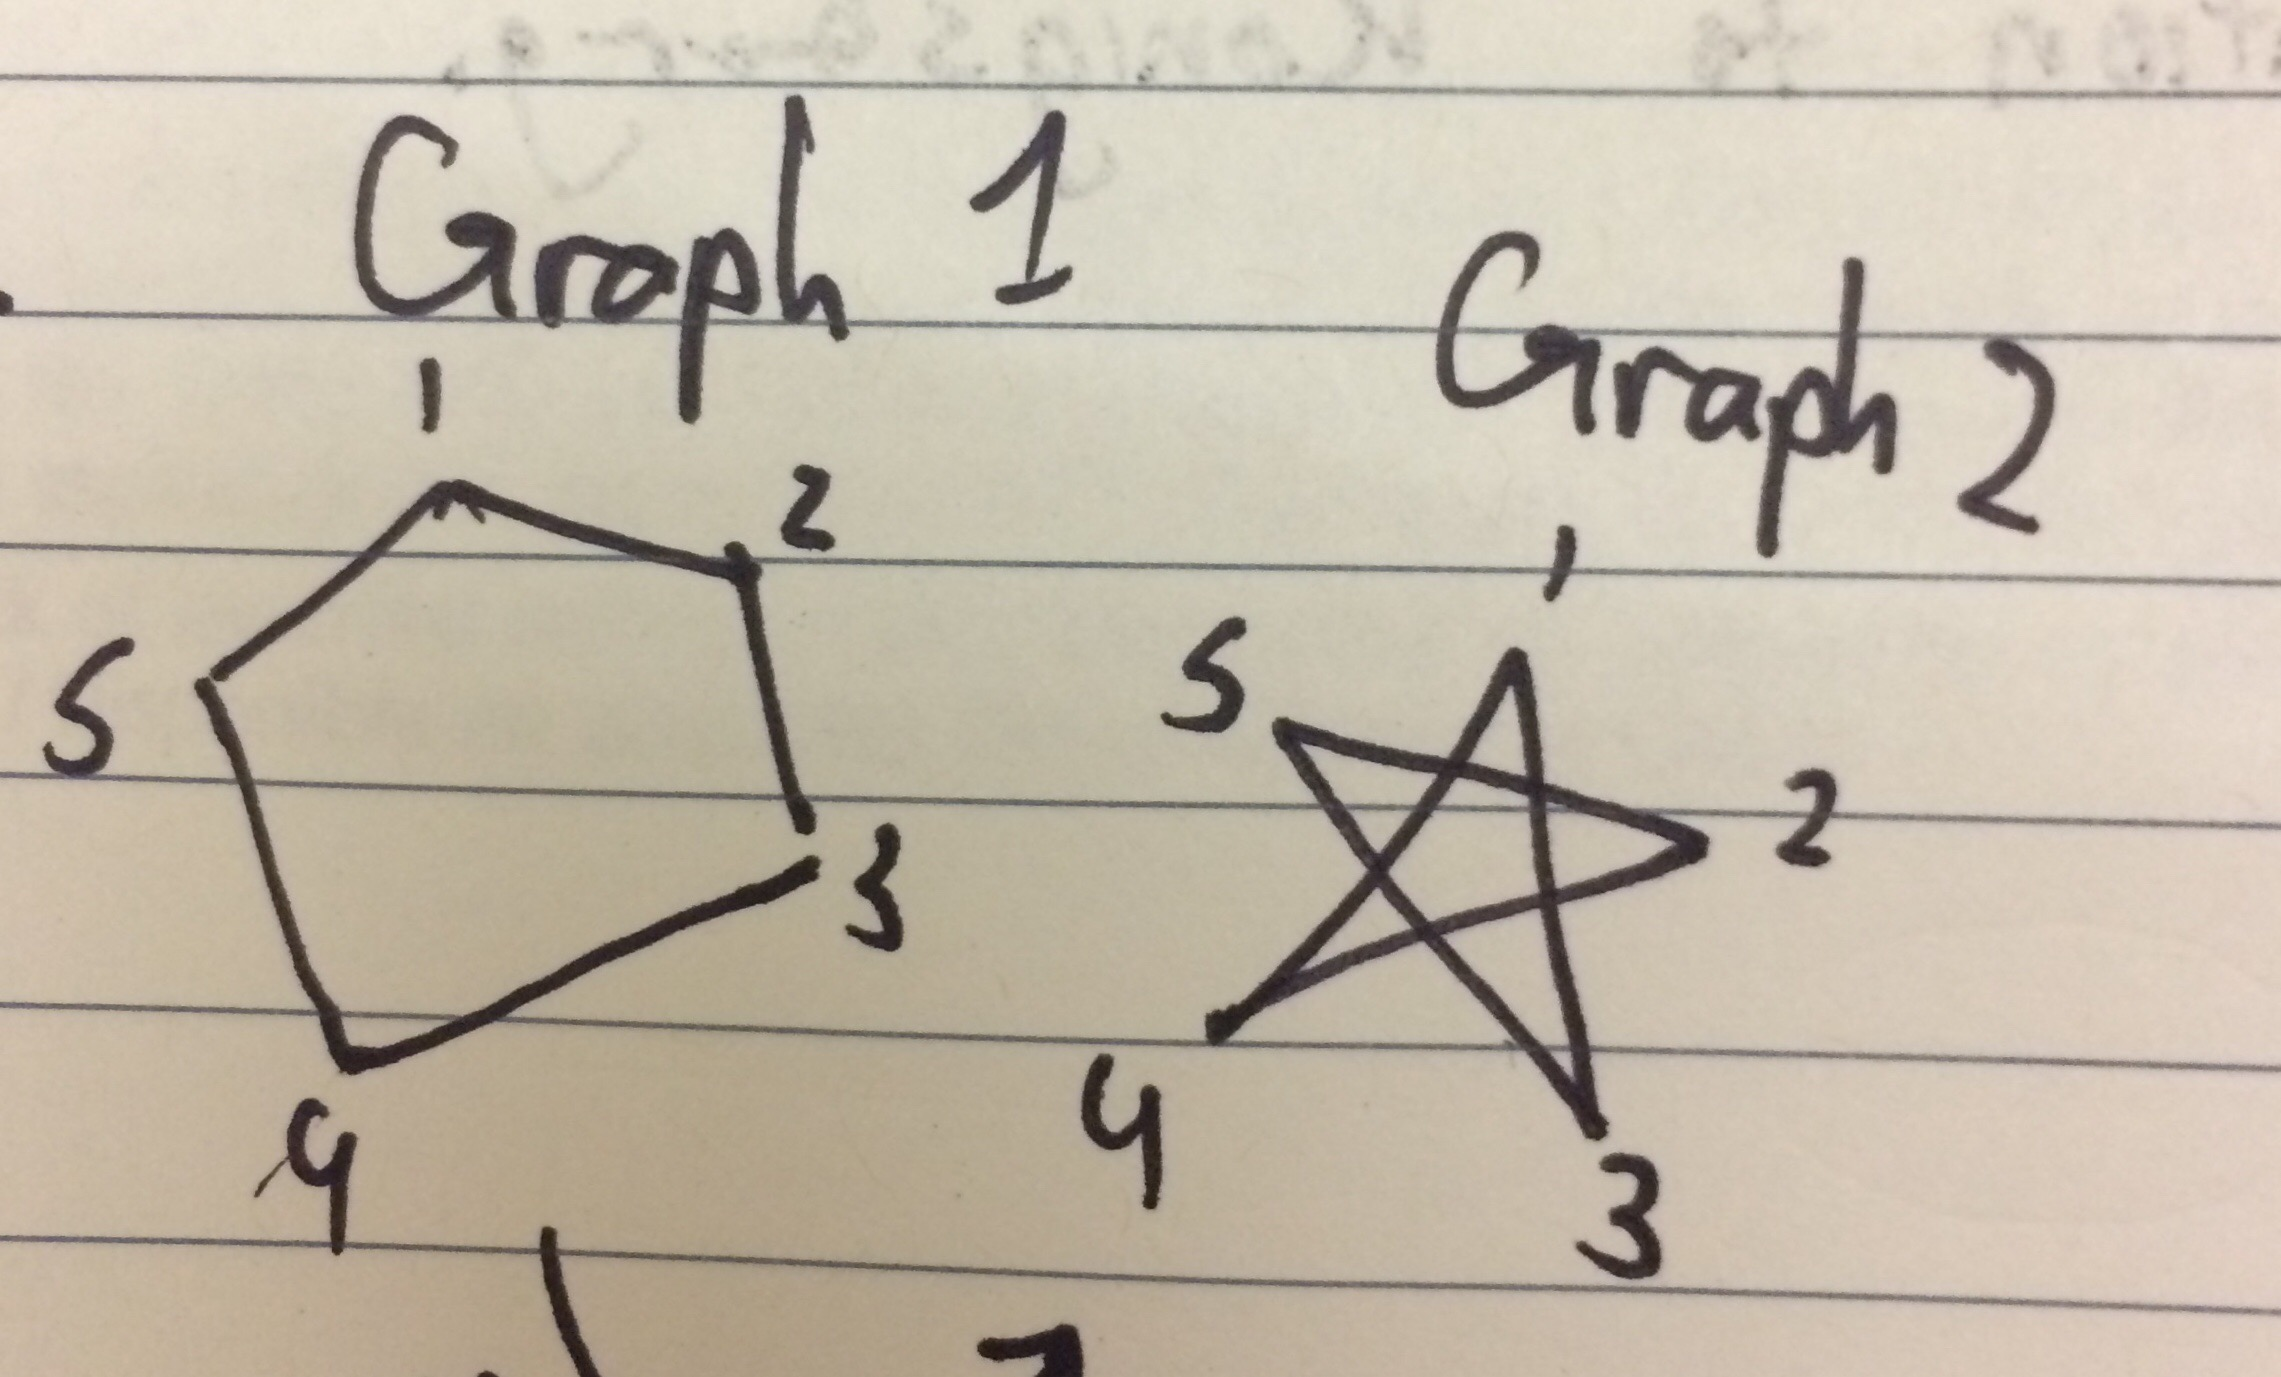
\includegraphics[scale=0.125]{lec3-1}\\
Graph 1 and Graph 2 are complements of each other.

We say a graph is \textbf{self-complementary} if a graph is isomorphic to its complement.

\subsection{Decomposing Graphs}

\begin{tcolorbox}[title=Definition: Union of Graphs]
	if $G_1, G_2$ are two graphs, assume $V(G_1), V(G_2) \subset V$ and $E(G_1), E(G_2) \subset E$. Then for a Graph $G_1 \cup G_2$
	\begin{itemize}
		\item{$V(G_1 \cup G_2) = V(G_1) \cup V(G_2)$}
		\item{$E(G_1 \cup G_2) = E(G_1) \cup E(G_2)$}
	\end{itemize}
\end{tcolorbox}

\underline{Example:}\\
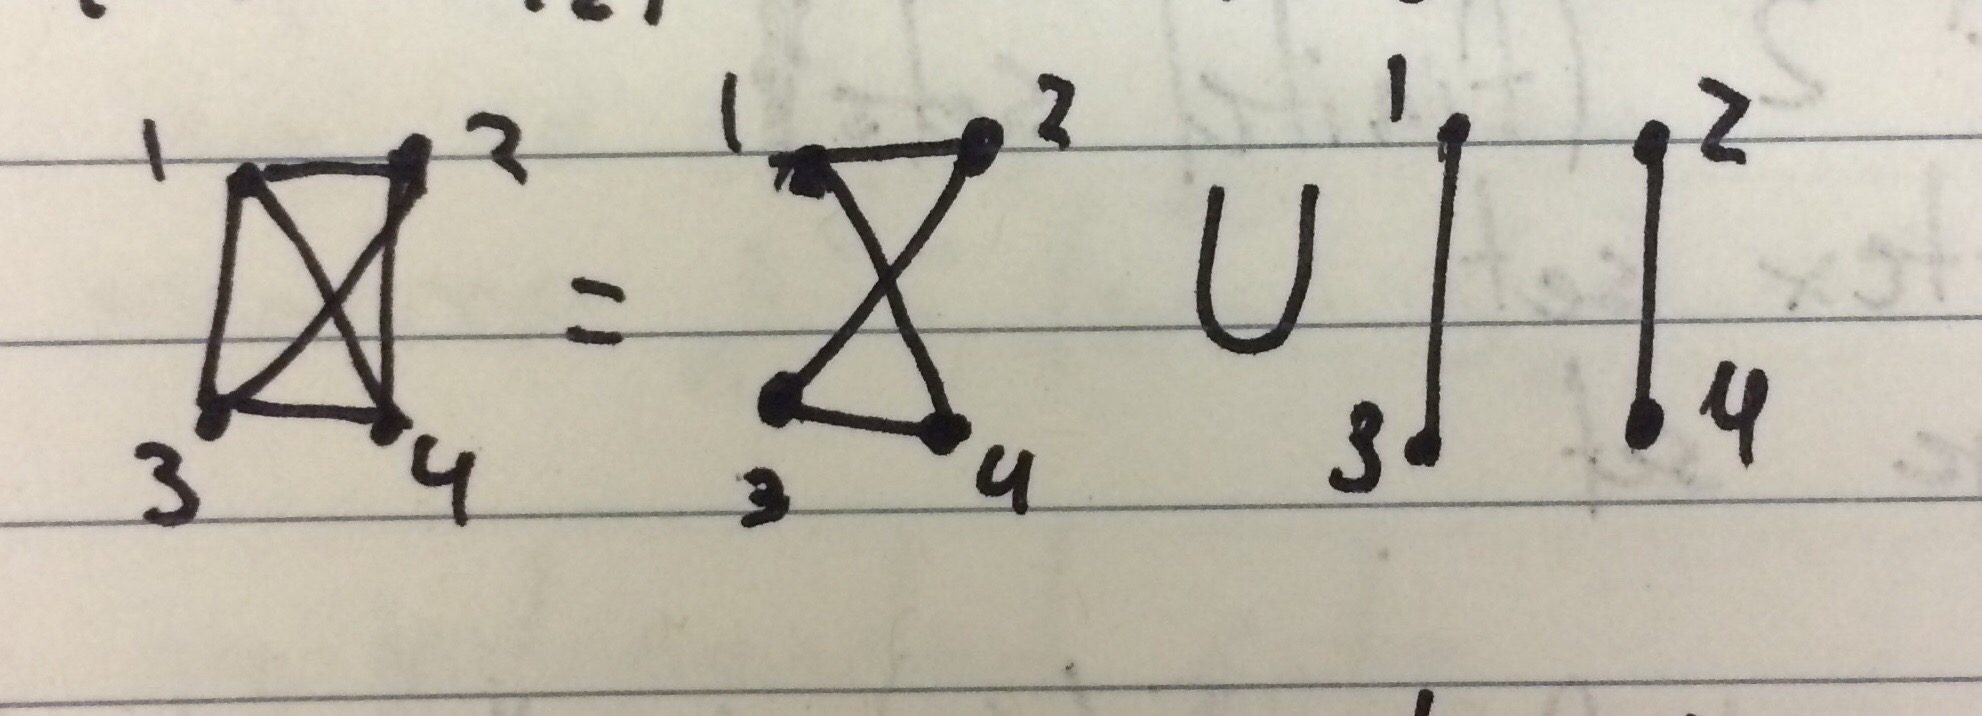
\includegraphics[scale=0.2]{lec3-2}\\

We say $G$ \textbf{decomposes} into $G_1$ and $G_2$ if the following:
\begin{itemize}
	\item{$G_1 \cup G_2 = G$}
	\item{if $\forall e \in E(G)$ there exists one $i$ such that $e\in E(G_i)$ (so if the edges between $G_1$ and $G_2$ don't overlap)}
\end{itemize}

\underline{Example:}\\
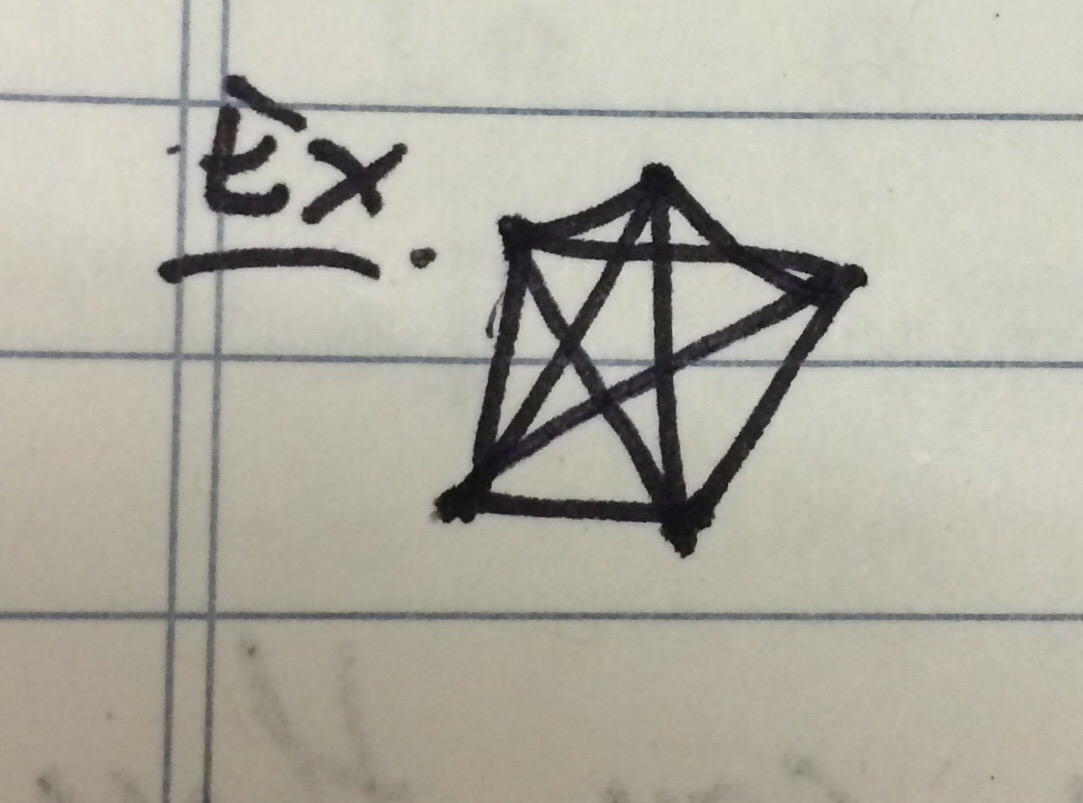
\includegraphics[scale=0.3]{lec3-3}\\
This is $k_5$, the complete simple graph of 5 vertices (complete meaning all vertices are adjacent)\\
\\
\underline{Example:}\\
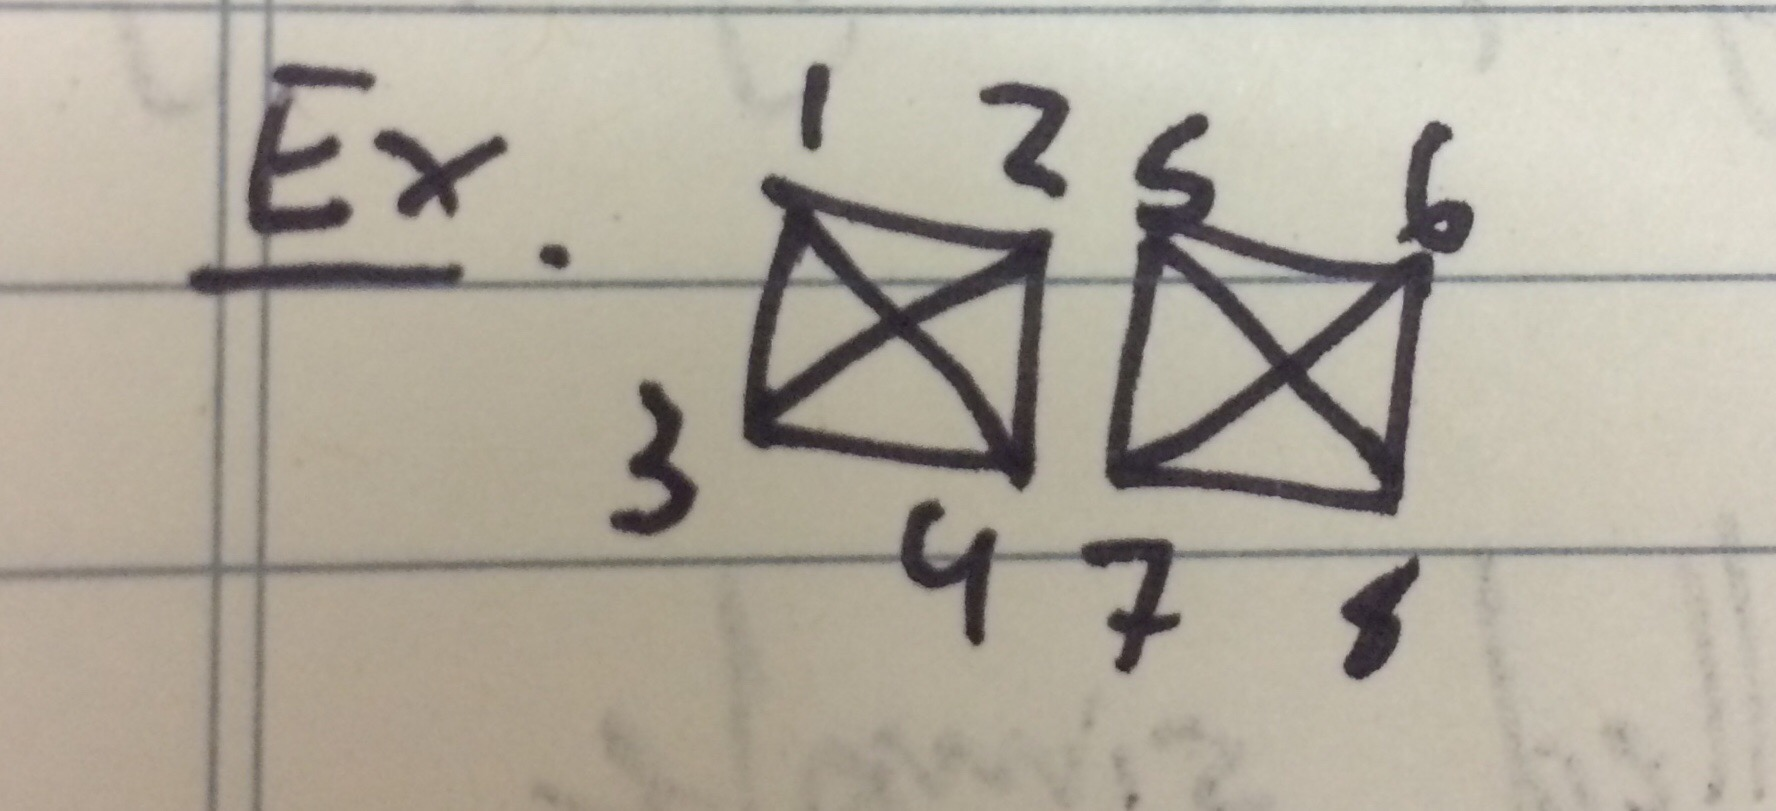
\includegraphics[scale=0.22]{lec3-4}\\
This is the disjoint union of 2 graphs. $G_1 \sqcup G_2$ is the union of 2 graphs with $V(G_1) \cap V(G_2) = \emptyset$

\subsubsection{Connectivity of $G$}

\paragraph{Path} A path is a simple subgraph such that we can order vertices $v_1, ... ,v_{n-1}$ in such a way that exactly $v_i, v_{i+1}$ are adjacent $\forall i$

\paragraph{Cycle} A cycle is a subgraph that is simple and that we the vertices $v_1, ... ,v_{n}$, $v_1 = v_n$ such that exactly $v_i, v_{i+1}$ are adjacent $\forall i$ and that all edges are unique.\\
\\

\underline{Note:} the arrangement of vertices in a path is called a \textbf{walk}, the arrangement of vertices in a cycle is called a \textbf{trail}.\\
\\
we refer to an edge by $(u,v)$ where $u,v$ are the start and end vertices.

\newpage

\section{Friday, September 15, 2017}

\subsection{Equivalence Relations on a set}

\underline{i.e.} Let $X$ be the set of people in a room and the pair $(p_1, p_2) \in R$ if $p_1 \in X$ and $p_2 \in X$ are the same age.\\
\\
An equivalence relation can be thought of as a certain property that is equal between 2+ elements.\\
\\
\begin{tcolorbox}
	\underline{Note:} For $R$ which is the set of people in $X$ that have the same age, you can subdivide $X$ into disjoint subsets of $R$. We can rename $R$ as $x_i$ where $i$ is the age of the people in the set (a partitioned $x$)
	$$\bigcup x_i = X$$
	$$x_i \cap x_j = \emptyset, i \neq j$$
\end{tcolorbox}

\begin{tcolorbox}[title=Definition: Equivalence Relation]
	A set of pairs $R$ is an equivalence relation if it has the following properties:
	\begin{itemize}
		\item{\textbf{Reflexive} : $\forall x \in X, (x,x) \in R$}
		\item{\textbf{Symmetric} : $\forall x,y \in X, (y,x) \in R$ implies $(y,x) \in R$}
		\item{\textbf{Transitive} : $\forall x,y,z \in X, (x,y),(y,z) \in R$ implies $(x,z) \in R$}
	\end{itemize}

\end{tcolorbox}

Some examples include people who like the same colour, have the same age, have the same major,....\\
\\
\underline{Claim:} If $R$ is an equivalence relation, then $X = \{ y : (x,y) \in R \}$ forms a partition.

\begin{proof}
	For notation, we will write $x \sim y$\\
	We need to prove 2 things.\\
	\begin{enumerate}
		\item{$\bigcup_{x\in X} \overset{\_\_\_}{x} = X$}, so we pick $x \in X$ and since $x \sim x$ then that implies that $x \in \overset{\_\_\_}{x}$
		\item{
			Union is disjoint. So we must prove that
			$$(a) \overset{\_\_\_}{x} \cap \overset{\_\_\_}{y} = \emptyset \text{ if } \overset{\_\_\_}{x} \neq \overset{\_\_\_}{y} \text{ iff } (b) \exists z : z\in \overset{\_\_\_}{x} \cup \overset{\_\_\_}{y} \rightarrow \overset{\_\_\_}{x} = \overset{\_\_\_}{y}$$
			
			If we assume $(b)$ is true then:
			\begin{align*}
				&\rightarrow x\sim z, y\sim z\\
				&\rightarrow x\sim z, z\sim y \text{ by symmetry}\\
				&\rightarrow x\sim y \text{ by transitivity}\\
				&\rightarrow y \in x
			\end{align*}
			next we assume $a\in\overset{\_\_\_}{x} \rightarrow x\sim a$, but $y\sim x \rightarrow y\sim a \rightarrow a \in y$
			Therefore we have that $\overset{\_\_\_}{x} \subset \overset{\_\_\_}{y}$ and $\overset{\_\_\_}{y} \subset \overset{\_\_\_}{x}$
		}
	\end{enumerate}
\end{proof}

\begin{tcolorbox}
	\textit{SideNote:} if we start with a partition of $X$ into subsets $(x)\in l $ then the relation $x\sim
y \leftrightarrow x,y$ lie in the same $X$ is an equivalence relation with partition $(x_i)_{i\in l}$
\end{tcolorbox}

\underline{Example:} Take the set of all graphs, say $G,G'$ and $\exists \text{ an isomorphism } G \mapsto G' $ and $G' \mapsto G''$ then $\exists \text{ an ismorphism }  g \circ f : G \mapsto G''$

\begin{tcolorbox}
	\textbf{Reminder:} graph $G$ with vertices $u,v$\\
	$(u,v) = $ path in a simple graph where we can order vertices $u,...,v$ such that only adjacent edges have consecutive endpoints (ordering is a walk)
\end{tcolorbox}

For any graph $G$, say $x,y \in V(G)$

$$x\sim y \leftrightarrow \begin{cases}
	y=x\\
	y \text{ is connected to } x
\end{cases}
$$
is an equivalence relation.\\
\\
For a vertex $v$, the set $\overset{\_\_\_}{v} = \{ y : y \text{ connected is the connected component of } x \text{ to } v \} $\\
\\
\begin{tcolorbox}
	\underline{Note:} The subgraph $\overset{\_\_\_}{x}$ is connected
\end{tcolorbox}

If $u_1, u_2 \in \overset{\_\_\_}{v}$ which imples that $u_1 \sim v, u_2 \sim v$ which implies that $u_1 \sim v, v \sim u_2$ which implies that $u_1 \sim u_2$

\begin{tcolorbox}
	\underline{Result:} Every graph is the disjoint union of common subgraphs, this result characterizes edge cuts and characterizes bipartite graphs
\end{tcolorbox}

\begin{tcolorbox}[title=Definition: Edge Cuts]
	In a graph $G$, an edge creates a cut if the number of connected components of $G \setminus \{ e \}$ increases
\end{tcolorbox}

If an edge lies in a cycle, it is not a cut edge or, a cut edge does not lie in a cycle.\\
\\
\begin{tcolorbox}[title=Thereom]
	An edge is a cut edge iff that edge does not lie on the cycle.
\end{tcolorbox}

\begin{proof}
	Take an edge $e$, we need to show that $G\setminus \{ e \}$ remains connected (which implies that e lies in a cycle).\\
	Assume $G \setminus \{ e \}$ is connected, let $x,y$ be the endpoints of $e$, since $G \setminus \{ e \}$ is connected, there is a path between $x,y \in G \setminus \{ e \}$.\\
	Now assume $e$ lies in a cycle in $G$, we need to show that $G \setminus \{ e \}$, or that there exists a path between nodes $u,v$ where $u$ is an adjacent node to $x$ but is not equal to $y$ and $v$ is an adjacent node to $y$ but is not equal to $x$.\\
	\\
	Now since $G \setminus \{ e \}$ is connected, there is a path between nodes $u$ and $v$ that does not go through edge $e$ and a path that goes through edge $e$ (namely, the path $u,x,y,v$). Therefore $e$ is not an edge cut iff it lies on a cycle. This implies that the negation of this is true, that an edge is an edge cut iff it doesn't lie on a cycle.
\end{proof}

\newpage

\section{Tuesday, September 19, 2017}

\subsection{Konig's Theorem (continued)}

\begin{tcolorbox}
	\underline{Recall:} Can we see when a given graph is bipartite? (A graph $G$ is bipartite if $V(G) = X \sqcup Y$ and $X,Y$ are independent sets)
\end{tcolorbox}

Konig's Theorem states that $G$ is bipartite iff there are no off length cycles.\\
\\
\textbf{Lemma:} In a graph $G$, any odd length walk that is also closed contains a cycle.\\
\\
From this we observe that we can assume that $G$ is connected.\\
\\
\underline{TONCAS (The Obvious Necessary Conditions Are Also Sufficient):} A bipartite graph cannot have odd length cycles.\\
\\
Observe that a cycle must travel through an even number of edges to return to the original vertex.\\
\\
\textit{Now consider the converse of this statement:} If the cycle travels odd edges, the cycle will be on the other side of the partition (so if $V(G) = X \sqcup Y$ and the cycle started at $X$, travelling odd edges will mean the cycle will finish in partition $Y$.)\\
\\
Let $v \in V(G)$\\
$X = \{ u \in V(G) : \text{ the path of minimal length between $v,u$ is even for all $v\in V(G)$ } \}$\\
$Y = \{ u \in V(G) : \text{ the path of minimal length between $v,u$ is odd for all $v\in V(G)$ } \}$
\\
\\
So we know from this that.
\begin{enumerate}
	\item{$G = X \sqcup Y $}
	\item{$X,Y$ are independent}
\end{enumerate}

Assume $X$ is not independent, so let $c$ be an edge between $u, u' \in X$, so take a path $$p: v \rightarrow u \text{ of minimal even length}$$ and a path $$p': u' \rightarrow v \text{ of minimal even length}$$
now consider the path $$v\overset{p}{\rightarrow} u \overset{c}{\rightarrow} u' \overset{p'}{\rightarrow} v$$
This is a closed walk of odd length, therefore there exists a closed cycle of odd length.\\
Therefore there exists a closed walk of odd length iff $X,Y$ are not independent (i.e. a Bipartite graph).

\subsection{Networks}

From this we will look at the Max Flow and Min Cut problem. This involves looking at directed graphs where all the edges in the graph are assigned a flow, which can represent the carrying capacity of trains along a route. This may be important as we may need to know what would be the best way to disrupt the network.

\begin{tcolorbox}[title=Definition: Directed Graph]
	A graph $G$ consists a set of vertices ($V(G)$) and a set of edges ($E(G)$) and
	$$E(G) \mapsto V(G) \times V(G) : e \mapsto (h(e), t(e))$$ where $h(e), t(e)$ refer to the head and tail of edge $e$ respectively.
\end{tcolorbox}

\begin{tcolorbox}[title=Definition: Network]
	A type of directed graph with a source node $s$ that no edge goes into and a sink node $t$ that no edge goes out of. There is also a capacity function $$c : E(G) \mapsto \mathbb{R} \geq 0$$ that assigns a capacity of flow for each edge in $E(G)$
\end{tcolorbox}

\begin{tcolorbox}
	\underline{Remark:} For this week, assume $G$ is simple directed graph, i.e. between any choice of $v_1,v_2 \in V(G)$, there exists at most 1 edge with a head of $v_1$ and a tail of $v_2$. We will also introduce some notation that if there exists an edge from $v_1$ to $v_2$ we denote it as $$v_1 \rightarrow v_2$$
\end{tcolorbox}

\begin{tcolorbox}[title=Definition: Capacity function]
	a capacity function $c: V \times V \mapsto \mathbb{R}\geq 0$ (takes in 2 vertices and returns a positive real number) and is defined by:
	$$c(v_1, v_2) = \begin{cases}
		c(v_1 \rightarrow v_2) &\text{ if }  (v_1 \rightarrow v_2)\in E\\
		0 &\text{ if }  (v_1 \rightarrow v_2)\not\in E\\
	\end{cases}
$$
\end{tcolorbox}
\begin{tcolorbox}[title=Definition: Flow $f$]
	a flow function is defined as $f: E(G) \mapsto \mathbb{R} \geq 0$ with the following properties:
	\begin{itemize}
		\item{$\forall e, f(e) \leq c(e)$}
		\item{for all vertexes v, $f^-(v) = \sum_{u \in V} f(u \rightarrow v)$}
		\item{for all vertexes v, $f^+(v) = \sum_{u \in V} f(v \rightarrow u)$}
		\item{$f^+(v) = f^-(v)$ for all vertices $v$ except for the sink and source nodes $s,t$}
	\end{itemize}
We also define $|f| = f^+(s)=f^-(t)$ as the value of the flow $f$
\end{tcolorbox}

\newpage

\section{Tuesday, September 26, 2017}

\subsection{Flow on a network}

So for some reason, Louis also denotes the value of the flow $f$ as $\partial f$.\\
\\
There are 2 main questions about network flows, and right now we will discuss the one in the form of the min-cut max-flow theorem.\\
\\
Starting from any flow, if it is not the maximal flow, we can construct one, but we must define a few terms first

\begin{tcolorbox}[title=Definition: Cut in a Network]
	Let $G$ be a network, a cut $(S,T)$ is a partition $V(G) = S \sqcup T$, where $s\in S, t \in T$. The \textit{capacity of the cut} is defined as
	$$\sum_{u\in S, v\in T} c(u,v) = c(S,T)$$
\end{tcolorbox}

\begin{tcolorbox}[title=Definition: Minimal Cut]
	Let $G$ be a network, a cut $(S,T)$ is a \textit{minimal cut} if $\forall (S', T')$ cuts of $G$, $$c(S,T) \leq c(S',T')$$
\end{tcolorbox}

\begin{tcolorbox}
	\underline{Recall:} for any flow $f$ and any cut $(S,T)$ on a graph $G$, $\partial f \leq c(S,T)$.\\
	We can also increase any flow until we get a maximum one from the Ford-Fulkerson algorithm.\\
	And for a maximum flow $f'$ and a minimal cut $(S',T')$, we get that $$\partial f' = c(S',T')$$
	Which is the min-cut, max-flow equation
\end{tcolorbox}

The Idea of the Ford Fulkerson Algorithm is that we use the appropriate paths from $s\rightarrow t$ to increase the flow of the network to the maximum flow accordingly.\\
\\
For a network $G$, a capacity function $c$ and a flow $f$.
\begin{itemize}
	\item{for any edge $(u,v)$ where $u,v \in V(G)$, the residual capacity of this edge is defined as $$c_f (u,v) = c(u,v) - f(u,v)$$}
	\item{An augmented path is an (undirected) path in the underlying graph $G$.}
	\item{For any edge, the residual capacity of that edge is strictly positive.}
\end{itemize}

Intuition for the Ford Fulkerson Algorithm:
\begin{enumerate}
	\item{if a flow has an augmented path, the flow cannot be maximal if the path goes from $s$ to $t$.}
	\item{If an augmented path $p$ between $s$ and $t$ exists, then we can adapt $p$ such that $\partial f$ increases and $p$ is no longer augmented.}
	\item{If there exists no augmented path $p$, this means that the path is maximal}
	\item{We use this construction to argue that there exists an obvious min-cut equal to the resulting value of the flow.}
\end{enumerate}

\underline{Example}, consider any path $p: s \rightarrow t$ on graph $G$, let $u,v$ be any 2 nodes in this path where $(u,v)$ is on the path.\\

let $m = \{ c_f (u,v) : (u,v) \in p \} = \{ c(u,v) - f(u,v) : (u,v) \in p \} > 0$ at each edge of the path $p$, replace $f(u,v)$ by $f(u,v) + m$\\
\\
Note that $\partial f$ has increased and that $p$ is no longer augmented.\\
\\
As if $m = c_f (u,v)$, the new flow has the weight of $$f(u,v) + m = f(u,v) + c(u,v) - f(u,v) = c(u,v)$$
\begin{tcolorbox}
	\underline{note:} Adding $m$ to all edges in p yields an increased flow.
\end{tcolorbox}

\newpage

\section{Friday, September 29, 2017}

\subsection{Max-flow Min-Cut Theorem (continued)}

The minimal amount needed of edges to remove is the maximum amount of flow of the network.\\
\\
Consider the capacity function: $$c: V \times V \mapsto \mathbb{R}$$
$$(u,v) \mapsto \begin{cases}
	c(u\rightarrow v) &\text{ if } u\rightarrow v \in E\\
	0 & \text{ otherwise}
\end{cases}$$

\begin{tcolorbox}[title=Theorem: Conservation]
	$$\partial f(v) = \sum f^+ (v) = \sum f^- (v)$$
	$$\partial f(v) = 0, \forall v \neq s,t$$
\end{tcolorbox}

In particular, the value of $f$ is $|f|=\partial f(s)$.

\begin{tcolorbox}[title=Min cut Max flow]
	\begin{itemize}
		\item{
		For any flow and any cut, $|f| \leq ||(S,T)||$ (this is the flow capacity inequality)\\
		$$|f| \text{ is max} \longleftrightarrow ||(S,T)|| \longleftrightarrow f \text{ is saturated for edges from $s$ to $t$}$$
		}
		\item{$G_f$, is the residual graph according to flow $f$}
		\item{If $G_f$ has no path from $s$ to $t$, then the flow is maximal}
		\item{(Ford-Fulkerson Algorithm) If there is a path in $G_f$ from $s$ to $t$, we can strictly increase the value of $|f|$ on $G$}
	\end{itemize}
\end{tcolorbox}

Start with the flow capacity inequality:
\textbf{Lemma} $|f| \leq ||(S,T)||$ for any flow $f$, cut $(S,T)$

$$|f| = \partial f(s) = f^+ (s) - f^- (s) = \sum_{u\in V} f(s \rightarrow u) - \sum_{u\in V} f(u\rightarrow s)$$

\textbf{Observation 1:} 

\begin{align*}
	\partial f(v) = 0 : \forall v \neq s,t \longrightarrow |f| &= \sum_{u\in V} f(s\rightarrow u)\\ 
	&= \sum_w f(w\rightarrow o) + \sum_{v \neq s} \partial f(v)\\
	&= \sum_{v \in S} (\sum_u f(v \rightarrow u) - \sum_w f(w\rightarrow v))
\end{align*}

\textbf{Observation 2:}

$$\sum_{v \in S} (\sum_u f(v\rightarrow u) - \sum_w f(w\rightarrow v)$$

Assume $u\in S$. For a choice of $v,u$ have the flow $f(v\rightarrow u)$ terminate.\\
\\
\begin{align*}
	&= \sum_{v\in S} (\sum_{u \in T} f(v\rightarrow u) - \sum_{w\int T} f(w\rightarrow v))\\
	&\leq \sum_{v\in S, u\in T} f(v\rightarrow u)\\
	&= ||(S,T)||
\end{align*}

Therefore, $|f|$ is maximal iff $||(S,T)||$ is minimal.

\begin{tcolorbox}
	\underline{Note:} \begin{itemize}
		\item{We say that $f$ saturates an edge if $f(u\rightarrow v) = c(u\rightarrow v)$}
		\item{We say that $f$ avoids an edge if $f(u\rightarrow v) = 0$}
	\end{itemize}

\end{tcolorbox}

So then $|f| = ||(S,T)||$ iff $f$ saturates any edge from $s$ to $t$ and avoids any edge from $t$ to $s$ (so all flows from $T$ to $S$ are 0). In this case, the flow is maximal.\\
\\
So we can say that the flow is maximal if every edge from $S$ to $T$ are saturated and every edge from $T$ to $S$ is avoided.

\begin{tcolorbox}[title=Definition: Residual Graph]
	\underline{residual capacity:} $$c_f : V \times V \mapsto \mathbb{R} \geq 0$$
	$$\begin{cases}
		c(u,v)-f(u,v) &\text{ if } (u,v) \in E\\
		f(u,v) &\text{ if } (v,u) \in E\\
		0 &\text{ otherwise}
	\end{cases}$$
	\underline{$G_f$, the residual graph:} Is a directed graph with
	$$\begin{cases}
		V(G_f) = V(G)\\
		(u,v) \in E(G_f) \text{ if } c_f(u,v) \neq 0
	\end{cases}$$
\end{tcolorbox}

\begin{tcolorbox}
	\underline{note:} If there is no path from $s$ to $t$ in $G_f$ then Let $S$ be the vertices reachable from $s$ (which also includes $s$) and let $T$ be the nodes $V(G_f) \setminus S$ (which also includes $t$). Then $(S,T)$ is a cut on $G$ or $G_f$
\end{tcolorbox}

Consider $u,v$ where $u\in S, v\in T$\\
we know that $c_f(u\rightarrow v) = 0$, since if it did, $v\in S$ which would be a contradiction of a cut.

$$c_f(u\rightarrow u) = c(u\rightarrow v) - f(u\rightarrow v) + f(u\rightarrow v) = 0 + 0 = 0$$

\underline{Conclusion:} There are no paths in $G_f$ from $s$ to $t$, this implies that the flow is maximal. i.e., $|f|=||(S,T)||$\\
\\
But what happens if $G_f$ has a path? We used that path $s\rightarrow t$ to increase the value of $f$ on $G$ (which is the Ford-Fulkerson Algorithm).\\
\\
As $s=u_1, u_2, ... , u_n = t$ is an "augmented" path $p$ on $G_f$ where $$\forall i : c_f(u_i, u_{i+1}) \neq 0$$
Let $F = min(c_f (u_i, u_{i+1}))$ on $G$, define a new flow $f'$ as follows.

$$f'(u\rightarrow v) =\begin{cases}
	f(u\rightarrow v) + F &\text{ if } u\rightarrow v \in p\\
	f(u\rightarrow v) - F &\text{ if } v\rightarrow u \in p\\
	f(u\rightarrow v) &\text{ otherwise}
\end{cases}
$$

\underline{Claim:} $f'$ is a flow on $G$ and $|f'|=|f|+F$
\begin{enumerate}
	\item{
	$\forall (u\rightarrow v) : f'(u\leftrightarrow v) \geq 0$ The only problem case where $u\rightarrow v$ in the path $p$ is $v\rightarrow u$ edge is in $G$ as subtracting $F$ made result in a flow smaller than 0.\\
	\\
	But calculating this out, we know that if $u\rightarrow v$ lies in the path $p$ and $F \leq f(u\rightarrow v) \forall u \rightarrow v$ in the path, so $f(u\rightarrow v) - F \geq 0$. So we know there is no problem as the flow always remains equal to or greater than 0.
	}
	\item{
	$\forall (u\rightarrow v) \in E(G) $ such that $f'(u\rightarrow v) \leq c(u\rightarrow v)$ but if $u\rightarrow v$ in the path, edge in $G$ 
	\begin{align*}
	f'(u\rightarrow v) &= f(u\rightarrow v) + F\\ 
	&= f(u\rightarrow v) + c(u\rightarrow v)\\
	&= c(u\rightarrow v) - (c_f(u\rightarrow v))\\
	&\leq c(u\rightarrow v)
	\end{align*}
	}
\end{enumerate}

\underline{Observation:} $|f'|=|f|+F$ since if the orientation changes, there is another adding edge that cancels out the subtracting edge, and otherwise, you add both adding edges.

\subsection{(Ford-Fulkerson) Algorithm for finding a maximal flow for a network}

\begin{enumerate}
	\item{start with original flow of f=0}
	\item{write down $G_f$}
	\item{choose a path on $G_f$ from $s\rightarrow t$ (if no path exists, the flow is maximal)}
	\item{increase the flow using this path, and repeat step 2 with new flow}
\end{enumerate}

\newpage

\section{Tuesday, October 3, 2017}

\subsection{Applying Min-cut Max-flow}

Say we want to prove a statement, that Graph $G$ has a set of edges with property $p$ or size $k$, as long as any set of vertices with property $q$ has size at least $k4$.\\
\\
\underline{Idea} To prove such a statement, we have to use the min-cut, max-flow theorem.
\begin{itemize}
	\item{Turn $G$ into a network, and let the flow value of the graph be $k$}
	\item{The graph should correspond to the set of edges with property $p$}
	\item{The set of $k$ vertices with property $Q$ corresponds to cut of capacity $k$}
	\item{There is a matching in $V(G)$, such that no 2 edges in the set share the same endpoint.}
\end{itemize}

\begin{tcolorbox}[title=Definition: Vertex Cover]
	Set of vertices $C$ such that any edge in $G$ has an endpoint of at least one vertex in $C$.
\end{tcolorbox}

\begin{tcolorbox}[title=Theorem: (Konig)]
	In a bipartite graph, There exists a matching of size $k$ as long as any vertex cover has at least size $k$.
	\tcblower
	Note that this variation of the definition of capacity includes $\infty$. i.e.
	$$c: V \times V \mapsto \mathbb{R}^+ \cup \{ \infty \}$$
	Even in this case, any finite flow has a max flow and a min cut. The point is to go from a bipartite graph to a network as such:
	\begin{center}
 \begin{tabular}{||c c||} 
 \hline
 Network & Bipartite Graph \\ [0.5ex] 
 \hline\hline
 flow & matching \\ 
 \hline
 value & size  \\
 \hline
 cut & vertex cover   \\
 \hline
 capacity & size \\ [1ex] 
 \hline
\end{tabular}
\end{center}
\end{tcolorbox}
\underline{i.e.}
\begin{enumerate}
	\item{Given a bipartite graph with $V(G) = X \sqcup Y$}
	\item{add an $s$ and $t$ node as the source and sink nodes respectively.}
	\item{connect every element of $s$ to $x$ and every element of $t$ to $y$ with an edge.}
	\item{Give a value of 1 to the capacity of the newly added edges, and a value of $\infty$ to the capacity of the original edges of the bipartite graph. }
\end{enumerate}

\underline{Conclusion 1:} any flow has a flow of $f(u,v)=\begin{cases}
1\\
0
\end{cases}$ for any edge $u\rightarrow v$

\underline{Conclusion 2:} if we look at a flow, and the subset of edges from $x$ to $y$ with $f(e)=1$. This is a matching. Note that any flow yields a matching.\\
\\
\underline{Conclusion 3:} Value of that flow is the number of edges in the matching.\\
\\
Understand cut capacities, Take a cut $(S,T)$, assume finite capacity $$c(S,T) = \sum_{u\in S, v\in T} c(u\rightarrow v)$$
Now, looking at $(X\cap T)\cup(Y\cap S)$, this is a vertex cover for $G$ edges between $X,Y$ such that the endpoints of the edges are not in the vertex cover set $C$.\\
\\
The first endpoint lies in $X \cap S$ and the second endpoint lies in $Y \cap T$. Because the edges now goes from $S$ to $T$ contributes to the capacity and $c(e)=\infty$.\\
\\
so a $(S,T)$ cut implies a vertex cover where the capacity of the cut is equal to the size of the vertex cover.
$$\sum_{u\in T} c(s,u) = \sum_{v\in S} c(v,t) = |C|$$

\underline{Conclusion:} A cut implies a vertex cover, the capacity of the cut is the size of the cover.\\
\\
And this finishes the proof by Max-Flow, Min-Cut.

\newpage

\section{Friday, October 6, 2017}

\subsection{Hall's Theorem on Perfect Matching}

Assume $|X| = |Y|$, does there exist a perfect match?\\
\\
Consider the marriage problem where nodes in $X$ represent women and nodes in $Y$ represent men.\\
\\
We require that for any $k$ women, they need to be interested (connected by an edge to) at least $k$ men (this is the sufficient condition).\\
\\
Let $G$ be a bipartite graph, $V(G) = X \sqcup Y$. $|X|=|Y|$.\\
\\
\begin{tcolorbox}[title=Marriage Condition]
	$W\subset X, \Gamma (W) = \{ y | (x,y)\in E, \text{ for some } x\in W \}$
\end{tcolorbox}
\begin{tcolorbox}[title=Theorem]
	The following are equivalent:
	\begin{itemize}
		\item{$G$ has a perfect matching}
		\item{$G$ satisfies the marriage condition.}
	\end{itemize}
\end{tcolorbox}

For a flow $f$, the value of $|f|$ is the size of the matching, if there exists a flow of value n. If there does not exist a flow of $|f|=n$. Produce a set $W \subset X$ such that $|W| > |\Gamma (W)|$ which implies that the max flow has a value of $k < n$.\\
\\
There exists a cut $(S,T)$ of capacity $||(S,T)||=k$
\begin{tcolorbox}
	\underline{note:} $(X\cap T) \cup (Y \cap S)$ is an edge cover of size k
\end{tcolorbox}
$$|X \cap T| + |Y \cap S| = k$$
$$|X \cap T| + |Y \cap S| = k < |X \cap T| + |X \cap S| = n$$
This is because $ |X \cap T| + |X \cap S| = |X|$ as max flow is $n$.\\
\\
This implies that $|Y\cap S| < |X \cap S|$.\\
\\
Take any $W = X \cap S$.\\
\\
For $W=X \cap S, \Gamma (W) \subset Y \cap S \longrightarrow |\Gamma (W)| < |W|$\\
\\
Any edge $(x,y)$ with $x \in (X \cap S)$ must have $y\in (X \cap S)$. If however $y \in (Y \cap T)$, edge $(x,y)$ contributes to the capacity of the cut, which in this case is of infinite capacity.\\
The Theorem is constructive: assume marriage condition is true, a max-flow implies a perfect matching (look at all edges between $X$ anad $Y$ with flow 1).

\subsection{Connectivity: Menger's Theorem}

\begin{tcolorbox}[title=Definition: edge-cut]
	Considering a connected graph $G$, we define an edge-cut as a set of edges $\{ e_1, ..., e_n \}$, such that removing these edges from the graph $G$ disconnects the graph.
\end{tcolorbox}

\begin{tcolorbox}[title=Definition: $k$-connected]
	We say $G$ is $k$-connected if the minimal size of the edge cut of $G$ is of size $k$.
\end{tcolorbox}

\underline{Example:} a $1$-connected graph means there exists at least one edge that is not lying on a cycle.\\
\\
\underline{Idea:} Menger's Theorem uses the Min-Cut Max-Flow theorem to extend this example.

\begin{tcolorbox}[title=Menger's Theorem]
	$G$ is $k$-connected iff any 2 points are connected by $k$ disjoint paths. The max size of a set of paths that are disjoint is $k$.
\end{tcolorbox}

This follows from the statement:\\
If $s,t$ are 2 vertices, what are the minimum amount of edges that need to be removed so that $s,t$ are disconnected from each other? This is the maximal cardinality of the set of $s\rightarrow t$ paths.\\
\\
This will follow from the version of the max-flow min-cut for directed graphs, but now given a directed graph, we create a network with a source node $s$ and a sink node $t$ with a capacity of 1 on all directed edges.

\newpage

\section{Tuesday, October 17, 2017}

\subsection{Planar Graphs}

To define planar and other concepts (i.e. 'faces'), we need a few definitions.

\begin{tcolorbox}[title=Definition: Open Ball]
	An open ball around point $x$ with radius $\epsilon$ is the set $$B(x,\epsilon ) = \{ y \in\mathbb{R}^n : ||y-x||<\epsilon \}$$
\end{tcolorbox}

\begin{tcolorbox}[title=Definition: Open set]
	An open set in $\mathbb{R}^n$ is a set $U$ such that $\forall x \in U$, there exists some ball $B(x,\epsilon ) \subset U$ for some $\epsilon > 0$
\end{tcolorbox}

\underline{counter-example:} the closed interval $[a,b]$ because for $b$, there does not exist an $\epsilon > 0$ such that $]b-\epsilon, b+\epsilon[ \subset [a,b]$, so $[a,b]$ is not an open set.\\
\\
More generally, a set that is not open is a closed disk.

\underline{Remark:} A contraction does not change a planar drawing. For example:
	
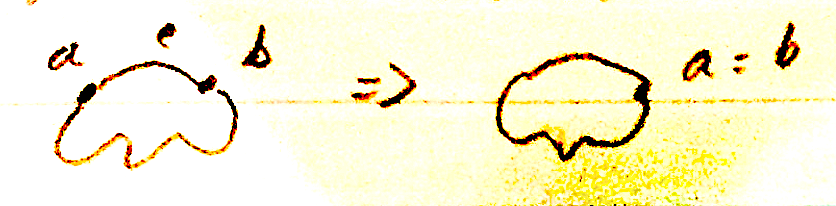
\includegraphics[scale=0.75]{lec10}

Here we just took edge $e$ and shrank it down. Thus, the planar graph $G$ retains the drawing.\\
\\
Using these 2 ingredients will help us prove Euler's Theorem.

\newpage

\section{Tuesday, October 24, 2017}

\subsection{Closed sets}

\begin{tcolorbox}[title=Definition: Closed Sets]
	For any set $x \in \mathbb{R}^n$, we define the closure of $x$ as follows.
	$$\overset{\_\_\_}{x} = \{ x \in \mathbb{R}^n : \text{ there exists a sequence in $x$, converging to } x \}$$
	In particular: $x\subset \overset{\_\_\_}{x}$, the set is closed if $\overset{\_\_\_}{x} = x$
\end{tcolorbox}

\underline{Example:} $[a,b]$ is closed, which converges as
$$a \leq \lim x_i \leq b$$ for any sequence $(x_i) \in [a,b]$\\
\\
\underline{Remark:} Closed means any sequence of elements in $X$ that converges has a limit in $X$\\
\\
\underline{Counter-Example:} $]a,b[$, Because we can find a sequence $(x_i)_{i\in l} \in ]a,b[$ converging to $b \not\in ]a,b[$. Take $x_i = b - \frac{1}{i}$

\begin{tcolorbox}[title=Relation between open and closed sets]
	The relation between open and closed sets is that
	$$\text{$X$ is open iff $X^c$ is closed}$$
\end{tcolorbox}

\underline{Remark:} Sets can be open, closed, or neither.\\
\underline{Example:} $]a,b[$ is an example of a set that is neither.

\newpage

\section{Friday, October 27, 2017}

\subsection{More Definitions for Planar Graphs}

\begin{tcolorbox}[title=Curve in $\mathbb{R}^n$]
	A curve in $\mathbb{R}^n$ is defined as a continuous function $$\gamma : [a,b] \mapsto \mathbb{R}^n$$
\end{tcolorbox}

\begin{tcolorbox}[title=Polygonal Curve]
	A polygonal curve is defined as a function
	$$\gamma : [a,b] \mapsto \mathbb{R}^n$$
	where $\exists a=a_0, a_1,..., a_n = b$ such that $\gamma [a_i,..., a_{i+1}]$ is a curve. 
\end{tcolorbox}

\begin{tcolorbox}[title=Drawing of a Graph]
	For a graph $G(V,E)$, the drawing of a graph is $f : V \mapsto \mathbb{R}^n$ and $f' : E\mapsto\text{ a polygonal curve in $\mathbb{R}^n$}$ such that if $e\in E$ is an edge with endpoints $a,b$, then this implies that $f'(e)$ is a curve from $f(a)$ to $f(b)$.
\end{tcolorbox}

This, for a planar graph with $n=2$ and for spherical drawing curves in a sphere, take values in $S^2 = \{ x : d(x,0)=1 \} \subset \mathbb{R}^3$.\\
\\
\underline{Example:} this is planar if you look at it directly, also one can see it as a cube with a cube section removed from it.\\
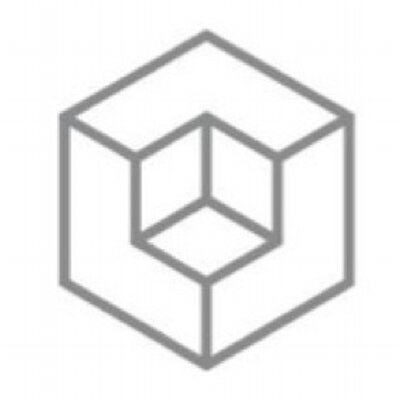
\includegraphics[scale=0.25]{lec12}

\begin{tcolorbox}
	\underline{Note:} Drawings of a graph are not invariant. There are multiple ways to draw a cube.
\end{tcolorbox}

\begin{tcolorbox}[title=Definition: Crossing of a graph]
	A crossing of a graph is defined as a point in $f(e) \cap f(e')$, where the point is not an endpoint of either $f(e)$ or $f(e')$
\end{tcolorbox}

\begin{tcolorbox}[title=Definition: Region in $\mathbb{R}^n$]
	An open set $\forall x,y$ in the region, there exists a polygonal curve with endpoints $x,y$ in the region.
\end{tcolorbox}

\begin{tcolorbox}[title=Definition: Face]
	\begin{enumerate}
		\item{Region of a graph drawing}
		\item{Does not interfere with intersect drawing}
		\item{maximal, i.e. another set $F'$ satisfies above properties and $F \subset F$ implies that $F = F'$}
	\end{enumerate}
\end{tcolorbox}

\begin{tcolorbox}[title=Euler's Formula]
	$$V-E+F=2$$
	For all planar graphs C that has a planar graph drawing, no crossing and must be connected. $F$ refers to the faces of the planar graph drawing.
\end{tcolorbox}

\underline{Example:} $V=4, E=6, F=4, 4-6+4=2$\\
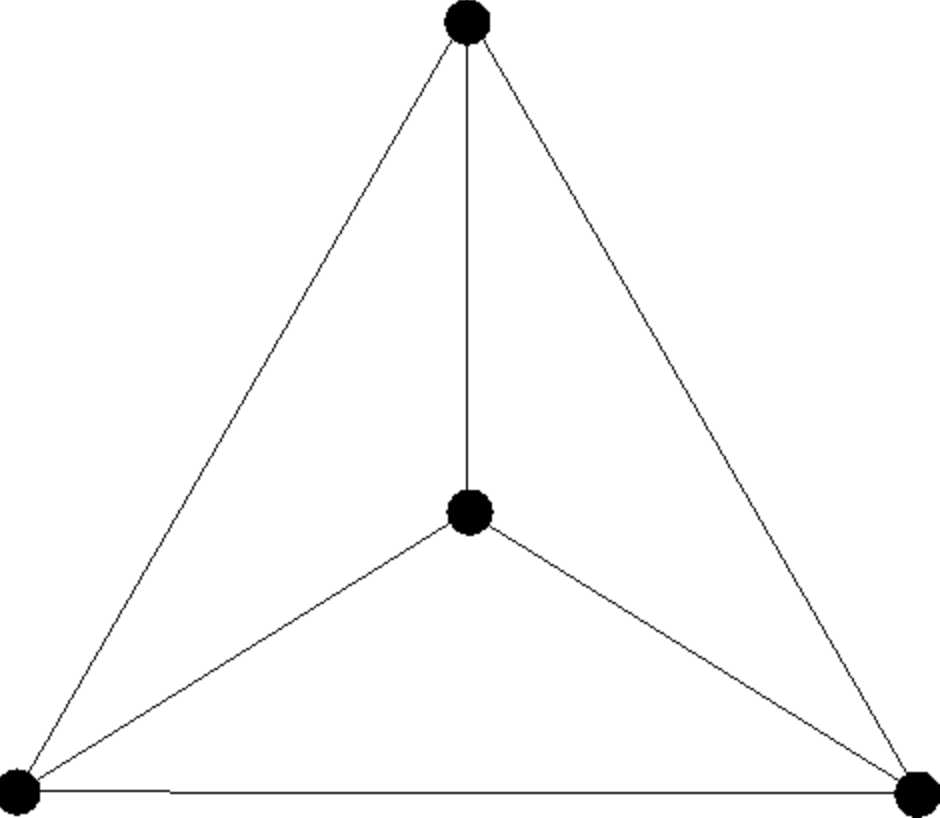
\includegraphics[scale=0.25]{lec12-1}

\begin{tcolorbox}[title=Definition: Jordan Curve Theorem]
	A curve that divides an area into two distinct regions (one on one side of the curve, and another on the other side of the curve.)
	Let $[a,b] \in \mathbb{R}^2$ (2 because there is no left or right in space) be a curve.
	A Jordan Curve is:
	\begin{enumerate}
		\item{A closed curve, i.e. $\gamma (a) = \gamma (b)$}
		\item{The curve $\gamma$ is simple (injective) (no point repeated).}
	\end{enumerate}
	$\gamma$ divides a region $R$ into 2 maximal regions with the boundary of $\gamma[a,b]$.
\end{tcolorbox}

\begin{tcolorbox}[title=Definition: Contraction of an edge]
	Consider an edge $e$, the contraction of an edge $e$ of a graph $G$ is the graph $G \setminus \{ e \}$ such that for the endpoint nodes $a,b$ of $e$, $a=b$
\end{tcolorbox}

\subsection{Planar Graphs}

\subsubsection{Application of Euler's formula for connected, planar graphs}

\begin{tcolorbox}
	\underline{Inequality 1:} For a planar graph with $V \geq 3$, $E \leq V-6$
\end{tcolorbox}

\begin{proof}
	Consider an arbitrary planar graph with $V \geq 3$.\\
	For each face, count the number of edges in the face. And since there as at least 3 edges in each face. Plugging this into Euler's formula we get
	\begin{align*}
		2E &\geq 3F\\
		F &\leq \frac{2}{3} E\\
		2 &= V-E+F \leq V-E+\frac{2}{3} E\\
		2 &\leq V - \frac{1}{3} E\\
		E &\leq 3V - 6
	\end{align*}
\end{proof}

\underline{Example:} Consider $K_5$ (graph with 5 nodes where there is an edge between any 2 vertices).\\
Note that this graph is not planar as $V=5, E=10$ and $10 \leq 3\cdot 5 - 6$ is not true.

\begin{tcolorbox}
	\underline{Inequality 2:} Assume $G$ has no triangles, then
	\begin{align*}
		2E &\geq 4F\\
		E &\geq 2F\\
		2 &= V-E+F \leq V-E+\frac{E}{2}\\
		4+E &\leq 2V\\
		E &\leq 2V - 4
	\end{align*}
\end{tcolorbox}

\underline{Example:} $K_{3,3}$, which is the bipartite graph where 
$$V = \{ x_1, ..., x_n \} \cup \{ y_1, ..., y_m \}$$
where any $x_i$ is connected to any $y_i$ by a single edge.\\

the result is $9 \not\leq 2\cdot 6 - 4$.

\section{Tuesday, October 31, 2017}

\subsection{Subdivisions}

\begin{tcolorbox}
	\underline{Recall:} For a planar connected graph
	\begin{itemize}
		\item{$V-E+F = 2$}
		\item{$E \leq 3V - 6$ (i.e., $K_5$ is not planar)}
		\item{$E \leq 2V - 4$ (i.e., $K_{3,3}$ is not planar)}
	\end{itemize}
\end{tcolorbox}

\begin{tcolorbox}[title=Definition: Elementary Subdivision of a graph $G$]
	An Elementary subdivision of graph $G$ is a new graph $G \sqcup \{ u \}$ where $u$ is placed onto an edge $e=(v,w)$ in the graph, so that the new edges are $(v,u), (u,w)$
\end{tcolorbox}
\begin{tcolorbox}[title=Definition: Subdivision of a graph $G$]
	A subdivision of graph $G$ is a graph obtained by 0 or more elementary subdivisions of $G$.
\end{tcolorbox}


Because of this definition, we can say that:\\
\textbf{If a graph is planar, then all of its subdivisions are planar}.\\
\\
A graph containing a subdivision of $K_5$ or $K_{3,3}$ then implies that the graph is not planar. This implication points both ways as well.

\begin{tcolorbox}[title=Kuratowski's Theorem]
	A graph is planar iff it does not contain a subgraph that is a subdivision of $K_5$ or of $K_{3,3}$
\end{tcolorbox}

\subsection{Dual Graphs}

Assume $G$ is planar, now consider a drawing of $G$ in a plane, the vertices of Dual Graph $G^*$ is equal to the faces of $G$ and there is an edge between $v_1, v_2 \in G^*$ if the face $v_1$ and the face $v_2$ have a common edge. The dual graph of a graph $G$ depends on the drawing of a graph $G$, so 2 different isomorphic graphs may have the same dual graph.\\
\\
We also know that: 
$$2|E| = \sum_{v \in V(G)} d(v)$$
Counting all the edges coming out of all vertices means that we double count every edge. But what happens when we apply this to $G^*$ instead.
$$G^*(V^*, E^*) \longrightarrow 2E^* = \sum_{v \in V*} d(v)$$
So now this equation means that all the edges that make up every face is being summed up.

\subsection{Platonic Solids}
A platonic solid is a solid where each face is a regular $k$-gon and there is the same amount of faces at any vertex.

\newpage

\section{Friday, November 3, 2017}

\subsection{Classifying Platonic Solids}

\textbf{Platonic Solid:} A solid such that each face is a regular $k$-gon and each vertex is adjacent to $l$-faces. \underline{ex.} a tetrahedron or a cube.\\
\\
All 5 platonic solids:\\
Tetrahedron -- made from triangles -- like a Pyramind\\
Octahedron -- Made from two pyramids put onto each other, made from triangles, like a diamond\\
Hexahedron (Cube)\\
Dodecahedron -- made from pentagons, soccerball\\
Icosahedron -- top and bottom are pyramids made from 5 triangles
\\
\\
\underline{Does any platonic solid has a planar graph?}

Let us look at the spherical embedding instead, since it does not make sense for the 3D representation to be a planar graph.

\begin{tcolorbox}[title=Definition: Spherical Embedding]
	Drawing of the graph $S^2 \subset \mathbb{R}^3$
\end{tcolorbox}

\underline{Geometric Fact:} The vertices of a platonic solid lie on a sphere, this means that any platonic solid has a spherical embedding without crossings.\\
\\
And the graph is spherical without crossing iff the graph is planar.\\
\\
This can be shown by drawing the stereographic projection, taking a point $P$ at the top of the sphere and a plane tangent to the bottom of the sphere, and the point $P$ will draw a stereographic projection by first intersecting with the edges and vertices of the sphere graph and onto the plane and that is where it is being projected. This produces a planar graph.\\
\\
This means that the image of a curve is a curve and if 2 curves cross in the plane, this implies that they must also cross on the sphere, and since the graph on the sphere is planar, the projection is also planar.\\
\\
\begin{tcolorbox}
	\underline{Recall:} For connected and planar graphs
	\begin{enumerate}
		\item{$2E = \sum_{F \text{ is a face}} e(F) = kF = lV$}
		\item{V-E+F=2}
	\end{enumerate}
\end{tcolorbox}

This implies that $$V = \frac{2}{l} E, F = \frac{2}{k} E$$ which implies that $$\frac{2}{l} E + \frac{2}{k} E - E = 2$$ which implies that $$E(\frac{2}{l} + \frac{2}{k} - 1) = 2$$ which implies that
\begin{align*}
	\longrightarrow& \frac{2}{l} + \frac{2}{k} - 1 > 0\\
	\longrightarrow& 2k +2l - kl > 0\\
	\longrightarrow& -2k -2l  + kl + 4 < 4\\
	\longrightarrow& (k-2)(l-2) < 4
\end{align*}

So this means that $k,l \geq 3$ and that only one platonic solid corresponds to each choice of $k,l$. So we get the result $3 \leq k, l \leq 5$ which only corresponds to the following pairs: $(3,3), (3,4), (4,3), (3,5), (5,3)$.

\subsection{Coloring}

Going forward, we will always consider the graph $G=(E,V)$ with gaps.
\begin{itemize}
	\item{A \textbf{colouring} by a set $C$ is defined as $c:V\mapsto C$}
	\item{This colouring is considered \textbf{proper} if no 2 adjecent vertices have the same colour}
	\item{Define a \textbf{Chromatic Number} $X^{(G)}$, for example: $$X^{(Petersen)}=3$$ And $X^{(G)} \leq n, n=|V|$ and $X^{(K_n)} = n$}
\end{itemize}

If $G$ has a colouring $c$, there is an equivalence relation such that $$v_1 \sim v_2 \text{ iff } c(v_1) = c(v_2) \text{ where } c \text{ is a colouring}$$ So we have the equivalence class $\overset{\_\_\_}{V}$ is the set of all vertices with the same colour.\\
\\
And if the colouring is proper, then the equivalence classes are independent as subgraphs.\\
\\
But what is the minimal size of a set $c$ with a proper colouring?\\
\\
\underline{conversely:} say $V$ is partitioned into subsets $C_1, C_2, ..., C_k$ where $$V=\sqcup^k_{i=1} C_i$$ Where each $C_i$ is the independent subgraph such that $$c:C \mapsto \{ 1,2,...,k \} \text{ where } v\mapsto i \text{ if } v \in C_i$$

\subsection{Bounds for colouring}

\underline{Recall} that a clique is a set of vertices whose induced subgraph is complete.

\subsubsection{Lower Bound}

Define $W(G)$ as the \textbf{size of the largest clique in $G$}.

\begin{tcolorbox}
	\underline{note:} $X(G) \geq W(G)$ because of $G$ is complete, then that implies that $X(G) = W(G)$.
\end{tcolorbox}

\underline{Argument:} Assume $G$ has a clique of size $l : v_1, ..., v_l$ then the subgraph induced by $v_1, ... ,v_l$ has the chromatic number $l$ where $l = W(G)$\\
Now note that $l = W(G)$.\\
Since $X(G) \geq X(G')$ for any subgraph $G'$.\\
Define $\alpha (G)$ as the size of the longest independent set of vertices.\\
$$X(G) \leq \frac{n}{\alpha (G)}, n=|V|$$
say $X(G) = l \longrightarrow$ $V$ can be paritioned into $l$ different independent sets, i.e. $l$ different sets of size $\leq \alpha (G)$\\
$\longrightarrow n \leq l, \alpha (G) = X(G)$.

\subsubsection{Upper Bound}

Start with greedy colouring (following is the steps for a greedy colouring algorithm).\\
$V = \{ v_1, ..., v_n \}$
\begin{itemize}
	\item{Assign colour $1$ to $v_1$}
	\item{If $v_2$ is not adjacent with $v_1$, colour it 1, otherwise, colour it 2}
	\item{If $v_3$ is not adjacent to $v_1$, then colour it 1, otherwise if not adjacent to $v_2$, colour it 2, otherwise, colour it 3.}
	\item{This goes on for every $v_i, \forall i : 1\leq i \leq n$}
\end{itemize}

\begin{tcolorbox}[title=Definition: Largest degree of a vertex in the graph $G$]
	$\Delta (G)$ is the largest degree of a vertex in the graph $G$, note that $X(G) \leq \Delta (G) + 1$
\end{tcolorbox}

\begin{tcolorbox}[title=Brook's Theorem]
	$X(G) \leq \Delta (G)$, unless $G$ is an odd cycle or $K_n$
\end{tcolorbox}

\newpage

\section{Tuesday, November 7, 2017}

\subsection{Colouring Problems}

Consider the function $c: V(G) \mapsto C$

\subsubsection{Lower Bound}

Recall that $\Delta (G)$ is the largest degree of a vertex in the graph $G$.\\
It is obvious to use that $\Delta (G) \leq X(G)$\\
So what is the role of $\Delta (G)$?\\
\\
We know for the upper bound that the greedy algorithm gives us a colouring with the smallest amount of colours. From that algorithm we concluded that $G$ has a colouring of $u+1$ colours as long as no $u$ predecessors are adjacent to $v_i$ for any $i$.\\
\\
In particular, $G$ always has a colouring of $\Delta (G) + 1$.
\begin{tcolorbox}[title=Brooke's Theorem]
	$X(G) \leq \Delta (G) + 1$ and $X(G) \leq \Delta (G)$ iff $G\neq \begin{cases}
		K_n\\
		\text{an odd cycle}
	\end{cases}
$
\end{tcolorbox}

We are only going to look at 2 cases when $\Delta (G) = k$:
\begin{enumerate}
	\item{Not all vertices have degree k}
	\item{the graph has a cut-vertex}
\end{enumerate}

(For 1), the idea is that we will used the greedy colouring algorithm with a clever ordering of the nodes. We will order the vertices $v_1, ... , v_n = V$ such that $d(v) < k$, so there are at most $k-1$ predecessors who are adjacent for each vertex.\\

\begin{tcolorbox}[title=Definition:Trees]
	Trees are a connected acyclic graph where any 2 vertices are connected by a single path.
\end{tcolorbox}

\begin{tcolorbox}[title=Definition: Spanning Tree]
	A spanning tree is a choice of edges such that the underlying graph is a tree for all nodes.
\end{tcolorbox}

\underline{Note:} Any connected graph $G$ has a spanning tree.

\begin{proof}
	(Proof any connected graph $G$ has a spanning tree)\\
	Use induction on the number of edges, which we will denote by $l$.
	\begin{enumerate}
		\item{$l=1$}
		\item{Assume any connected graph of  $|E|\leq l$  has a spanning tree, Now consider the graph with $l+1$ edges. We can pick any $e\in E(G)$. Now consider the case when $e$ does not lie on a cycle, that would mean that $G \setminus e$ is not connected, which implies that $G \setminus e$ has 2 connected conponents $G_1 \sqcup G_2$, which implies that each graph has their own spanning trees ($T_1, T_2$ respectively) since they both have  $\leq l$ edges. And to finish this proof, we need to show that $T_1 \cup T_2 \cup e $ is a spanning tree.}
	\end{enumerate}
\end{proof}

\newpage

\section{Tuesday, November 14, 2017}

\subsection{5-Colour Theorem}

\begin{tcolorbox}
	\underline{Recall:} that the \textbf{6-colour theorem} stating that every planar graph has a 6-colouring is easy because by Euler's formula, there exists a vertex with degree $\leq 5$, so this implies the result.
\end{tcolorbox}

So what about the 5-colour theorem?\\
\\
Consider the graph with the node $u$ connected to 5 nodes, labelled $a,b,c,d,e$ clockwise. Assume that all nodes connected to $u$ all have a distinct colour (Lets say $c(a)=1, c(b)=2, c(c)=3, c(d)=4, c(e)=5$). Now consider the subgraph of all vertices, coloured $1,3$ connected to the node $c$ (we will call this subgraph $G_1$), and consider the subgraph of all vertices, coloured $1,3$ connected to the node $a$ (we will call this subgraph $G_2$).\\
\\
\textbf{Scenario 1:} vertices $a,c$ are not connected, because if so, then $G_1, G_2$ are not disjoint in $G$, but we can make it work by simply alternating the colouring of the nodes of one of the trees from $3 \leftrightarrow 1$.\\
\\
If we remain with a proper colouring by colouring the node $u$ with the colour 3. This is only not proper if there exists a node $v$ connected to $G_1$ that is the same colour as the node it is connected to. This is impossible as $v$ would be in $V(G_1)$ and would not be the same colour as it would have its colour changed.\\
\\
\textbf{Scenario 2:} vertices $a,c$ are connected, so we cannot change the colours. Now we will look at:
\begin{itemize}
	\item{$G_2 : $ subgraph of $\forall u \in V(G_2)$ connected to node $b$}
	\item{$G_4 : $ subgraph of $\forall u \in V(G_4)$ connected to node $d$}
\end{itemize}

but now these graphs must cross an edge but cannot connect, so \textit{scenario 1} must apply to $G_2, G_4$.\\
\\
\underline{Question 1:} What is the smallest proper colouring we can find?\\
\underline{Question 2:} How many colourings are there?\\
\\
Consider the birthday problem. On a graph, its assigning colours $\{ 1,...,365 \}$ to nodes to represent $n$ people. ($K_n$).\\
\\
For $n$ people, it's colouring of $K_n$ is the possible combinations, where there is an edge between 2 nodes if they have a unique bday.\\
\\
For a room of 23 people, the probability of 2 people sharing the same birthday is $52\%$, and 70 people results in a probability of $99\%$.\\
\\
This is why we may be interested in how many colourings there are.\\
\\
\begin{tcolorbox}[title=Definition: Chromatic Polynomial]
	For a graph $G$ and an positive integer $t$, $$P(G, t) = \text{ The number of proper $t$-colourings on $G$}$$
\end{tcolorbox}

\underline{Example 1:} For $n$ vertices without any edges, $$P(G,t) = t^n$$
\underline{Example 2:} For $K_n$, $$P(K_n, t) = \frac{t!}{(t-n)!}$$

\underline{Why is $P(G,t)$ a polynomial and how to compute it?}\\
\\
Recall that contracting an edge $e=(u,v)$ is removal of the edge $e$ and $u=v$. Where the graph with the edge $e$ is contracted is graph $G_e$.

$$P(G,t) = P(G \setminus e,t) - P(G_e, t)$$

The differences between $G \setminus e$ and $G_e$ is that $u,v$ can be the same colour in $G \setminus e$ but not in $G$. But in $G_e$, $u,v$ are the same node and therefore the same colour, so the equation holds.\\
\\
\underline{$P(G,T)$ is a polynomial}

\begin{proof}
	(Induction on the number of edges)\\
	\textbf{Base Case:} If there are no edges, we know that $P(G,T) = t^n$\\
	\\
	\textbf{Induction Step:} $G_e$ and $G \setminus e$ are polynomials, and a polynomial subtract a polynomial is still a polynomial.
\end{proof}

\newpage

\section{Friday, November 17, 2017}

\subsection{Graph Colouring}

\underline{Recall:} Chromatic Polynimals are $P(G,t)$.\\
\\
There are 2 applications:
\begin{enumerate}
	\item{Supposed we want the Chromatic number of the cycle $P(C_3, t) = t(t-1)(t-2)$}
	\item{
	$C_4 : P(C_4, t) = t(t-1)^2 (t-2) + t(t-1)^2$\\
	For $C_4$, there are 2 ways to colour it. Treat pairs in a bipartite split with different colours (2 colours) and setting all of the vertices as different colours.
	}
\end{enumerate}

\underline{General Result for Cycles:} $$P(C_n, t) = (t-1)^n + (-1)^n (t-1)$$
Proof that result agrees with above:\\
$$e \in C_n, C_n \setminus \{ e \} = \Pi_n \rightarrow (C_n)_e = C_{n-1}$$
\begin{proof}
	(Proof by Induction)\\
	\textbf{Base Case:} $n=3$, $P(C_3, t) = t(t-1)(t-2) = (t-1)^3 - (t-1)$
	\textbf{Induction Step:} By induction, assume the format is true for any $n$-cycle.\\
	Then:
	\begin{align*}
		P(C_{n+1},t) &= P(\Pi_{n+1}, t) - P(C_n, t)\\
		&= t(t-1)^n - ((t-1)^n + (-1)^n (t-1))\\
		&= (t-1)^n (t-1) - (-1)^{n+1} (t-1)\\
		&= (t-1)^{n+1} - (-1)^{n+1} (t-1)
	\end{align*}
\end{proof}

This also applies for any tree (which are all connected and acyclical).

\begin{tcolorbox}
	\underline{Remark:} Any tree has a vertex with degree $> 1$ (if $|E| > 1$)
\end{tcolorbox}
\begin{proof}
	(Proof by induction on the number of edges)\\
	\textbf{Base Case:} For a connected tree with only 2 edges, one vertex must have a degree of 2.\\
	\textbf{Induction Step:} Assume this holds for all trees with $|E|=n$, Consider a tree with $|E|=n+1$. Just remove any edge $e$, so $G\setminus e$ is a union of trees with less than $n$ edges, and therefore must have the statement be true.\\
	Therefore by induction, every tree has a vertex of at least degree 2.
\end{proof}

Let $e$ be an edge with endpoint node $v$ ($deg(v)=1$). Then 
$$T_n \setminus \{ e \} = T_{n-1} \sqcup \{ v \}, (T_n)' = T''_n$$
\begin{proof}
	(Proof by induction on edges)\\
	\textbf{Base Case:} $E=1$, $P(T_2, t) = t(t-1)^{2-1}$\\
	\textbf{Induction Step:} Assume formula holds for any tree with $n$ vertices.\\
	Then 
	\begin{align*}
		P(T_{n+1}, t) &= P(T_n \sqcup \{ v \}, t) - P(T_n'', t)\\
		&= t P(T_n', t) - P(T_n'',t)\\
		&= t(t(t-1)^{n-1}) - t(t-1)^{n-1}\\
		&= t(t-1)^n
	\end{align*}
\end{proof}

\subsection{Spanning Trees}

\underline{motivating question:} How should Toronto plow snow as efficiently as possible?\\
\\
i.e. For a graph $G$, highlight edges such that:
\begin{itemize}
	\item{Each vertex in the graph is some endpoint for some edge}
	\item{There does not exist a path between 2 vertices}
\end{itemize}

\begin{tcolorbox}[title=Definition: Spanning Tree]
	For a connected graph $G$, a spanning tree is a subgraph $T$ which is a tree, $V(T)=V(G)$
\end{tcolorbox}
\begin{tcolorbox}[title=Definition: Weighted graph]
	A weighted graph is a graph $G$ with a weight function $$w : E(G) \mapsto \mathbb{N}$$
\end{tcolorbox}
\begin{tcolorbox}[title=Definition: Minimum Spanning Tree]
	A minimum spanning tree is a spanning tree where the sum of weights on edges is minimal among all possible spanning trees.
\end{tcolorbox}

\subsubsection{Finding a Minimum Spanning Tree}

\begin{enumerate}
	\item{Prim's Algorithm}
	\item{Kruskal's Algorithm}
\end{enumerate}

\begin{tcolorbox}[title=Kruskal's Algorithm]
	Kruskal's Algorithm is a greedy algorithm, meaning that it takes the most optimal decision at each step individually to get the most desired result once the algorithm concludes.
	\begin{enumerate}
		\item{Order edges by increasing edge weight}
		\item{Highlight lowest value edges such that no cycle is created}
		\item{Will end up with a minimum spanning tree once all nodes are covered}
	\end{enumerate}
\end{tcolorbox}

Assume $T \subset G$ is a spanning tree.\\
$e \in E(G \setminus T) \longrightarrow T \cup \{ e \}$ is no longer a tree (we have introduced a cycle), so $T \cup \{ e \}$ has a unique cycle (since $T$ initially did not have a cycle).

\begin{proof}
	(Proof of result)\\
	We first observe that:\\
	\begin{enumerate}
		\item{The algorithm results in a spanning tree}
		\item{Any choice of edges in the algorithm is part of a minimum spanning tree}
	\end{enumerate}
So lets look at these observations. We know the result is acyclic because the algorithm does not choose edges that create cycles. We also know that the result is connected because if no, pick 2 connected components in $G$, the components are connected at some point an edge with minimum weight will connect components in $T$.
\end{proof}

\newpage

\section{Tuesday, November 21, 2017}

This lecture was simply looking at different algorithms for looking for minimum spanning trees and an example of them running on a graph.

\subsection{Kruskal's Algorithm}

This algorithm is essentially ordering all the edges by edge weight, and then adding the edge one by one if they did not create a cycle. We continue adding edges until we get a Minimum Spanning Tree 

\subsection{Prim's Algorithm}

We start by picking a node and we choose the smallest connected edge until we get a Minimum Spanning Tree

\subsection{Dijkstra's Algorithm}

We find the minimum weight of a $u\rightarrow v$ path for a graph $G$ with nodes $u,v \in V(G)$.

\newpage

\section{Friday, November 24, 2017}

\subsection{Spanning Cycles -- Eulerian Cycles}

Let a graph $G$ have a cycle $C$ where $E(G) = C$ and $V(G) = C$.

\begin{tcolorbox}[title=Definition: Eulerian Path \slash  Cycle]
	An eulerian path is a path that goes through each edge once. An eulerian cycle is an eulerian path that is a cycle.
\end{tcolorbox}

\underline{Examples of eulerian cycles:}
\begin{itemize}
	\item{Joint cycles}
	\item{A single cycle}
\end{itemize}

Supposed $G$ is a connected graph, if an eulerian $C$ is plausible on $G$, then $G$ can be decomposed into cycles.

\begin{tcolorbox}[title=Definition: $G$ can be decomposed into cycles]
	if $E(G) = E(C_1) \sqcup ... \sqcup E(C_n)$ where each $C_i$ is a simple cycle.
\end{tcolorbox}

(For now) Assume:\\ 
\paragraph{Theorem} $G$ is Eulerian iff $G$ can be decomposed into cycles.
\paragraph{Theorem} $G$ is Eulerian iff all vertices have an even degree.

\underline{Proof Checklist:}
\begin{enumerate}
	\item{$G$ Eulerian implies all vertices have an even degree}
	\item{All vertices have an even degree implies $G$ is eulerian}
	\item{$G$ Eulerian iff  $G$ can be decomposed into cycles.}
\end{enumerate}

\begin{tcolorbox}
	\underline{Note:} An even graph is a graph with nodes all of an even degree.
\end{tcolorbox}

\paragraph{Lemma} If the degree of all vertices is $\geq 2$ then $v$ contains a cycle.
\begin{proof}
	Take a maximal path between 2 vertices $u,v$ so that $p: u=v_1,...,v_n=v$ and maximal in the sense that there is no edge between $v_n$ and some $v_{n+1}$, such that $v_1,...,v_n, v_{n+1}$ is a path.
\end{proof}

\underline{Going down proof checklist:}
\begin{enumerate}
	\item{$G$ is Eulerian implies that evert vertex degree is even goes back to the 7 bridges problem.}
	\item{
	if all vertices have an even degree, this implies that $G$ is eulerian.
	\begin{proof}
		Induction on $n$ simple cycles in $G$ where $n\geq 1$.\\
		\textbf{Base Case: $n=1$}, is trivial\\
		\textbf{Induction Step:} Assume this works for $k$ simple cycles.\\
		$G$ is eulerian implies that $G$ is an even graph containing $k$ simple cycles, take a graph $G$ without even degree vertices, which contain $k+1$ simple cycles. If we remove simple cycle $C$, then $G \setminus C$ has $k$ simple cycles and even degree vertices.
	\end{proof}
	}
\end{enumerate}

\newpage

\section{Tuesday, November 28, 2017}

\subsection{Hamiltonian Paths \slash  Cycles}

\begin{tcolorbox}[title=Definition: Hamiltonian Path \slash  Cycle]
	An hamiltonian path is a path that goes through each node once. An hamiltonian cycle is an hamiltonian path that is a cycle.
\end{tcolorbox}

\begin{tcolorbox}
	\underline{Note:} A Hamiltonian cycle implies a hamiltonian path since a hamiltonian cycle is a path.
\end{tcolorbox}

\underline{Example:} A cycle is an example of a Hamiltonian Cycle
\begin{itemize}
	\item{$G$ is hamiltonian implies $G'$ is hamiltonian if $V(G') = V(G)$ and $E(G') \supseteq E(G)$}
	\item{A non example would be a cycle that can be decomposed into 2 simple cycles.}
	\item{Another example would be $K_n$}
\end{itemize}

If $G$ is bipartite, $G$ may be Hamiltonian.\\
If $G$ is bipartite and hamiltonian, that implies that $|X|=|Y|$ where $V(G) = X \sqcup Y$

\subsubsection{Necessary Conditions}

Assume $G$ has a hamiltonian cycle. This means that $G$ is at least 2-connected.

\subsubsection{Sufficient Conditions}

\paragraph{Theorem} if $d(v) \geq \frac{|V|}{2}$ for all vertices $v\in V$ then this implies that $G$ has a Hamiltonian Cycle (for $|V| \geq 3$).

\begin{tcolorbox}
	\underline{note:} This bound is tight, there exists graphs where $d(v) = \frac{|V|}{2} -1$ that are not Hamiltonian.
\end{tcolorbox}

Consider a hamiltonian graph $G$ with adjacent vertices $u,v$ implies that $G + uv$ is Hamiltonian. The converse is only sometimes true.

\newpage

\section{Friday, December 1, 2017}

\subsection{Hamiltonian Graphs}

\begin{tcolorbox}[title=Definition: Hamiltonian Graphs]
	A graph $G = (V,E)$ contains a a Hamiltonian cycle (cycle with the vertex set $V$).
\end{tcolorbox}

This is different when compared to an Eulerian graph.\\ 
\\
Let's say $G$ is Hamiltonian, add an edge $e$ anywhere, $G \cup \{ e \}$ is Hamiltonian.\\
\\
Let's say $G$ is Hamiltonian, add an edge $e$ between non-adjacent nodes, $G \cup \{ e \}$ is never Eulerian.\\
\\
Consider $G$ as an even graph ($d(v)$ is even for all $v\in V$)

\subsubsection{Necessary Condition} 

The graph $G$ is bipartite and $|X| = |Y|$ as well as 2-connected.

\subsubsection{Sufficient Condition} 

\paragraph{Dirac's Theorem} That $\forall v \in V, d(v) \geq \frac{|V|}{2}$ implies that the graph $G$ is hamiltonian

\begin{tcolorbox}
	\underline{remark:} For 2 adjacent vertices $u,v$, $d(v) + d(u) \geq |V|$, this implies that $G \setminus \{ e=(u,v) \}$ remains Hamiltonian
\end{tcolorbox}

\paragraph{Ore's Theorem} For 2 adjacent vertices $u,v$, $d(v) + d(u) \geq |V|$, this implies that $G \setminus \{ e=(u,v) \}$ remains Hamiltonian (rephrase of Dirac)

Now consider the graph $G$, $\forall u,v \in V$ that are non-adjacent, if $d(u) + d(v) \geq |V|$, Consider $G \cup \{ e=(u,v) \}$. Repeat until no such edges remain, this is the \textbf{closure} of $G$

\begin{tcolorbox}[title=Bondy-Chvatal Theorem]
	$G$ is hamiltonian iff $\overset{\_\_\_}{G}$ is hamiltonian
\end{tcolorbox}


\end{document}



























